\documentclass[twoside]{book}

% Packages required by doxygen
\usepackage{fixltx2e}
\usepackage{calc}
\usepackage{doxygen}
\usepackage{graphicx}
\usepackage[utf8]{inputenc}
\usepackage{makeidx}
\usepackage{multicol}
\usepackage{multirow}
\PassOptionsToPackage{warn}{textcomp}
\usepackage{textcomp}
\usepackage[nointegrals]{wasysym}
\usepackage[table]{xcolor}

% NLS support packages
\usepackage[french]{babel}

% Font selection
\usepackage[T1]{fontenc}
\usepackage{mathptmx}
\usepackage[scaled=.90]{helvet}
\usepackage{courier}
\usepackage{amssymb}
\usepackage{sectsty}
\renewcommand{\familydefault}{\sfdefault}
\allsectionsfont{%
  \fontseries{bc}\selectfont%
  \color{darkgray}%
}
\renewcommand{\DoxyLabelFont}{%
  \fontseries{bc}\selectfont%
  \color{darkgray}%
}
\newcommand{\+}{\discretionary{\mbox{\scriptsize$\hookleftarrow$}}{}{}}

% Page & text layout
\usepackage{geometry}
\geometry{%
  a4paper,%
  top=2.5cm,%
  bottom=2.5cm,%
  left=2.5cm,%
  right=2.5cm%
}
\tolerance=750
\hfuzz=15pt
\hbadness=750
\setlength{\emergencystretch}{15pt}
\setlength{\parindent}{0cm}
\setlength{\parskip}{0.2cm}
\makeatletter
\renewcommand{\paragraph}{%
  \@startsection{paragraph}{4}{0ex}{-1.0ex}{1.0ex}{%
    \normalfont\normalsize\bfseries\SS@parafont%
  }%
}
\renewcommand{\subparagraph}{%
  \@startsection{subparagraph}{5}{0ex}{-1.0ex}{1.0ex}{%
    \normalfont\normalsize\bfseries\SS@subparafont%
  }%
}
\makeatother

% Headers & footers
\usepackage{fancyhdr}
\pagestyle{fancyplain}
\fancyhead[LE]{\fancyplain{}{\bfseries\thepage}}
\fancyhead[CE]{\fancyplain{}{}}
\fancyhead[RE]{\fancyplain{}{\bfseries\leftmark}}
\fancyhead[LO]{\fancyplain{}{\bfseries\rightmark}}
\fancyhead[CO]{\fancyplain{}{}}
\fancyhead[RO]{\fancyplain{}{\bfseries\thepage}}
\fancyfoot[LE]{\fancyplain{}{}}
\fancyfoot[CE]{\fancyplain{}{}}
\fancyfoot[RE]{\fancyplain{}{\bfseries\scriptsize Généré le Mardi 2 Décembre 2014 14\+:26\+:07 pour Dessinator\+: client par Doxygen }}
\fancyfoot[LO]{\fancyplain{}{\bfseries\scriptsize Généré le Mardi 2 Décembre 2014 14\+:26\+:07 pour Dessinator\+: client par Doxygen }}
\fancyfoot[CO]{\fancyplain{}{}}
\fancyfoot[RO]{\fancyplain{}{}}
\renewcommand{\footrulewidth}{0.4pt}
\renewcommand{\chaptermark}[1]{%
  \markboth{#1}{}%
}
\renewcommand{\sectionmark}[1]{%
  \markright{\thesection\ #1}%
}

% Indices & bibliography
\usepackage{natbib}
\usepackage[titles]{tocloft}
\setcounter{tocdepth}{3}
\setcounter{secnumdepth}{5}
\makeindex

% Hyperlinks (required, but should be loaded last)
\usepackage{ifpdf}
\ifpdf
  \usepackage[pdftex,pagebackref=true]{hyperref}
\else
  \usepackage[ps2pdf,pagebackref=true]{hyperref}
\fi
\hypersetup{%
  colorlinks=true,%
  linkcolor=blue,%
  citecolor=blue,%
  unicode%
}

% Custom commands
\newcommand{\clearemptydoublepage}{%
  \newpage{\pagestyle{empty}\cleardoublepage}%
}


%===== C O N T E N T S =====

\begin{document}

% Titlepage & ToC
\hypersetup{pageanchor=false,
             bookmarks=true,
             bookmarksnumbered=true,
             pdfencoding=unicode
            }
\pagenumbering{roman}
\begin{titlepage}
\vspace*{7cm}
\begin{center}%
{\Large Dessinator\+: client \\[1ex]\large 1.\+0.\+0 }\\
\vspace*{1cm}
{\large Généré par Doxygen 1.8.8}\\
\vspace*{0.5cm}
{\small Mardi 2 Décembre 2014 14:26:07}\\
\end{center}
\end{titlepage}
\clearemptydoublepage
\tableofcontents
\clearemptydoublepage
\pagenumbering{arabic}
\hypersetup{pageanchor=true}

%--- Begin generated contents ---
\chapter{Index hiérarchique}
\section{Hiérarchie des classes}
Cette liste d'héritage est classée approximativement par ordre alphabétique \+:\begin{DoxyCompactList}
\item \contentsline{section}{Angle}{\pageref{class_angle}}{}
\item \contentsline{section}{Connexion}{\pageref{class_connexion}}{}
\item \contentsline{section}{Couleurs}{\pageref{class_couleurs}}{}
\item \contentsline{section}{Dessinable}{\pageref{class_dessinable}}{}
\begin{DoxyCompactList}
\item \contentsline{section}{Dessin\+Manager}{\pageref{class_dessin_manager}}{}
\end{DoxyCompactList}
\item \contentsline{section}{Erreur}{\pageref{class_erreur}}{}
\item \contentsline{section}{Expert$<$ retour, a\+Traiter $>$}{\pageref{class_expert}}{}
\begin{DoxyCompactList}
\item \contentsline{section}{Expert\+C\+O\+R$<$ retour, a\+Traiter $>$}{\pageref{class_expert_c_o_r}}{}
\end{DoxyCompactList}
\item \contentsline{section}{Expert$<$ Forme\+Geom, string $>$}{\pageref{class_expert}}{}
\begin{DoxyCompactList}
\item \contentsline{section}{Expert\+C\+O\+R$<$ Forme\+Geom, string $>$}{\pageref{class_expert_c_o_r}}{}
\begin{DoxyCompactList}
\item \contentsline{section}{Expert\+Chargement}{\pageref{class_expert_chargement}}{}
\begin{DoxyCompactList}
\item \contentsline{section}{Chargement\+Cercle}{\pageref{class_chargement_cercle}}{}
\item \contentsline{section}{Chargement\+Groupe}{\pageref{class_chargement_groupe}}{}
\item \contentsline{section}{Chargement\+Polygone}{\pageref{class_chargement_polygone}}{}
\item \contentsline{section}{Chargement\+Segment}{\pageref{class_chargement_segment}}{}
\item \contentsline{section}{Chargement\+Triangle}{\pageref{class_chargement_triangle}}{}
\end{DoxyCompactList}
\end{DoxyCompactList}
\end{DoxyCompactList}
\item \contentsline{section}{Facade$<$ retour, a\+Traiter $>$}{\pageref{class_facade}}{}
\item \contentsline{section}{Facade$<$ Forme\+Geom, string $>$}{\pageref{class_facade}}{}
\begin{DoxyCompactList}
\item \contentsline{section}{Chargement\+Facade}{\pageref{class_chargement_facade}}{}
\end{DoxyCompactList}
\item \contentsline{section}{Matrice\+Carree2}{\pageref{class_matrice_carree2}}{}
\item \contentsline{section}{Objet\+Geom}{\pageref{class_objet_geom}}{}
\begin{DoxyCompactList}
\item \contentsline{section}{Forme\+Geom}{\pageref{class_forme_geom}}{}
\begin{DoxyCompactList}
\item \contentsline{section}{Cercle}{\pageref{class_cercle}}{}
\item \contentsline{section}{Forme\+Composee$<$ C, T $>$}{\pageref{class_forme_composee}}{}
\item \contentsline{section}{Forme\+Composee$<$ Forme\+Geom, Groupe $>$}{\pageref{class_forme_composee}}{}
\begin{DoxyCompactList}
\item \contentsline{section}{Groupe}{\pageref{class_groupe}}{}
\end{DoxyCompactList}
\item \contentsline{section}{Forme\+Composee$<$ Point, Polygone $>$}{\pageref{class_forme_composee}}{}
\begin{DoxyCompactList}
\item \contentsline{section}{Polygone}{\pageref{class_polygone}}{}
\end{DoxyCompactList}
\item \contentsline{section}{Segment}{\pageref{class_segment}}{}
\item \contentsline{section}{Triangle}{\pageref{class_triangle}}{}
\end{DoxyCompactList}
\item \contentsline{section}{Point}{\pageref{class_point}}{}
\end{DoxyCompactList}
\item Q\+Main\+Window\begin{DoxyCompactList}
\item \contentsline{section}{Main\+Window}{\pageref{class_main_window}}{}
\end{DoxyCompactList}
\item \contentsline{section}{Vecteur}{\pageref{class_vecteur}}{}
\end{DoxyCompactList}

\chapter{Index des classes}
\section{Liste des classes}
Liste des classes, structures, unions et interfaces avec une brève description \+:\begin{DoxyCompactList}
\item\contentsline{section}{\hyperlink{class_angle}{Angle} \\*The \hyperlink{class_angle}{Angle} class Classe représentant un angle. On l'instancie avec un angle exprimé en degré }{\pageref{class_angle}}{}
\item\contentsline{section}{\hyperlink{class_cercle}{Cercle} \\*The \hyperlink{class_cercle}{Cercle} class Cette classe représente un cercle, c'est à dire un point pour le centre et un double représentant le rayon }{\pageref{class_cercle}}{}
\item\contentsline{section}{\hyperlink{class_chargement_cercle}{Chargement\+Cercle} }{\pageref{class_chargement_cercle}}{}
\item\contentsline{section}{\hyperlink{class_chargement_facade}{Chargement\+Facade} }{\pageref{class_chargement_facade}}{}
\item\contentsline{section}{\hyperlink{class_chargement_groupe}{Chargement\+Groupe} }{\pageref{class_chargement_groupe}}{}
\item\contentsline{section}{\hyperlink{class_chargement_polygone}{Chargement\+Polygone} }{\pageref{class_chargement_polygone}}{}
\item\contentsline{section}{\hyperlink{class_chargement_segment}{Chargement\+Segment} }{\pageref{class_chargement_segment}}{}
\item\contentsline{section}{\hyperlink{class_chargement_triangle}{Chargement\+Triangle} }{\pageref{class_chargement_triangle}}{}
\item\contentsline{section}{\hyperlink{class_connexion}{Connexion} \\*The \hyperlink{class_connexion}{Connexion} class Cette classe est charg�e d'�tablire une connexion avec un serveur distant Cette classe charge une seule fois les dll Windows pour toutes les instances, cette partie est donc un singleton. De plus elle est compilable et fonctionnelle sous windows et unix(linux / mac compris) car la portabilit� c'est la vie }{\pageref{class_connexion}}{}
\item\contentsline{section}{\hyperlink{class_couleurs}{Couleurs} \\*The \hyperlink{class_couleurs}{Couleurs} class Cette classe représente les différentes couleurs disponible dans l'application et contient les différentes méthodes utiles pour les manipuler }{\pageref{class_couleurs}}{}
\item\contentsline{section}{\hyperlink{class_dessinable}{Dessinable} \\*The \hyperlink{class_dessinable}{Dessinable} class Il s'agit d'une interface décrivant le comportement que doivent avoir les classes de dessin. Cette classe sers donc majoritairement à assurer l'évolutivité de l'application en indiquant aux autres classes voulant dessiner les formes géometriques quelles méthodes elles doivent implémenter }{\pageref{class_dessinable}}{}
\item\contentsline{section}{\hyperlink{class_dessin_manager}{Dessin\+Manager} \\*The \hyperlink{class_dessin_manager}{Dessin\+Manager} class Cette classe est chargé de dessiner les formes géometriques. Le dessin est fait en envoyant les formes géometriques à un serveur distant afin que celui-\/ci dessine }{\pageref{class_dessin_manager}}{}
\item\contentsline{section}{\hyperlink{class_erreur}{Erreur} }{\pageref{class_erreur}}{}
\item\contentsline{section}{\hyperlink{class_expert}{Expert$<$ retour, a\+Traiter $>$} }{\pageref{class_expert}}{}
\item\contentsline{section}{\hyperlink{class_expert_chargement}{Expert\+Chargement} }{\pageref{class_expert_chargement}}{}
\item\contentsline{section}{\hyperlink{class_expert_c_o_r}{Expert\+C\+O\+R$<$ retour, a\+Traiter $>$} }{\pageref{class_expert_c_o_r}}{}
\item\contentsline{section}{\hyperlink{class_facade}{Facade$<$ retour, a\+Traiter $>$} }{\pageref{class_facade}}{}
\item\contentsline{section}{\hyperlink{class_forme_composee}{Forme\+Composee$<$ C, T $>$} }{\pageref{class_forme_composee}}{}
\item\contentsline{section}{\hyperlink{class_forme_geom}{Forme\+Geom} }{\pageref{class_forme_geom}}{}
\item\contentsline{section}{\hyperlink{class_groupe}{Groupe} \\*The \hyperlink{class_groupe}{Groupe} class Un groupe est un ensemble de formes composées. Chaque forme le constituant est une copie de la forme originale. L'ajout d'une forme dans un groupe change sa couleur pour celle du groupe }{\pageref{class_groupe}}{}
\item\contentsline{section}{\hyperlink{class_main_window}{Main\+Window} }{\pageref{class_main_window}}{}
\item\contentsline{section}{\hyperlink{class_matrice_carree2}{Matrice\+Carree2} }{\pageref{class_matrice_carree2}}{}
\item\contentsline{section}{\hyperlink{class_objet_geom}{Objet\+Geom} }{\pageref{class_objet_geom}}{}
\item\contentsline{section}{\hyperlink{class_point}{Point} }{\pageref{class_point}}{}
\item\contentsline{section}{\hyperlink{class_polygone}{Polygone} \\*The \hyperlink{class_polygone}{Polygone} class Cette classe représente un poygone, c'est à dire une ensemble de points dans un ordre donné. Un polygone contient au moins trois points. Les points stockés dans un polygone sont des copies des points envoyés. L'ordre dans lequel on ajoute les points correspond à l'ordre dans lequel ils seront reliés\+: si on insère un point dans un polygone, il sera relié à au dernier point inséré et au premier de la liste }{\pageref{class_polygone}}{}
\item\contentsline{section}{\hyperlink{class_segment}{Segment} }{\pageref{class_segment}}{}
\item\contentsline{section}{\hyperlink{class_triangle}{Triangle} }{\pageref{class_triangle}}{}
\item\contentsline{section}{\hyperlink{class_vecteur}{Vecteur} }{\pageref{class_vecteur}}{}
\end{DoxyCompactList}

\chapter{Documentation des classes}
\hypertarget{class_angle}{\section{Référence de la classe Angle}
\label{class_angle}\index{Angle@{Angle}}
}


The \hyperlink{class_angle}{Angle} class Classe représentant un angle. On l'instancie avec un angle exprimé en degré.  




{\ttfamily \#include $<$angle.\+h$>$}

\subsection*{Fonctions membres publiques}
\begin{DoxyCompactItemize}
\item 
\hypertarget{class_angle_a82d90a585c6e52fbe5514e6c1b327cbe}{{\bfseries Angle} (const double degre)}\label{class_angle_a82d90a585c6e52fbe5514e6c1b327cbe}

\item 
\hypertarget{class_angle_ae22d147ca274e7958800df1a21291021}{double {\bfseries get\+Radian} () const }\label{class_angle_ae22d147ca274e7958800df1a21291021}

\item 
\hypertarget{class_angle_ad10cc86bfb48bb9ebbc4c758552e51b1}{double {\bfseries get\+Degre} () const }\label{class_angle_ad10cc86bfb48bb9ebbc4c758552e51b1}

\end{DoxyCompactItemize}
\subsection*{Attributs publics statiques}
\begin{DoxyCompactItemize}
\item 
\hypertarget{class_angle_adb021f735de596a5d1a665d1a14ff7b9}{static constexpr double {\bfseries P\+I} = 3.\+14159265359}\label{class_angle_adb021f735de596a5d1a665d1a14ff7b9}

\end{DoxyCompactItemize}


\subsection{Description détaillée}
The \hyperlink{class_angle}{Angle} class Classe représentant un angle. On l'instancie avec un angle exprimé en degré. 

La documentation de cette classe a été générée à partir du fichier suivant \+:\begin{DoxyCompactItemize}
\item 
angle.\+h\end{DoxyCompactItemize}

\hypertarget{class_cercle}{\section{Référence de la classe Cercle}
\label{class_cercle}\index{Cercle@{Cercle}}
}


The \hyperlink{class_cercle}{Cercle} class Cette classe représente un cercle, c'est à dire un point pour le centre et un double représentant le rayon.  




{\ttfamily \#include $<$cercle.\+h$>$}

Graphe d'héritage de Cercle\+:\begin{figure}[H]
\begin{center}
\leavevmode
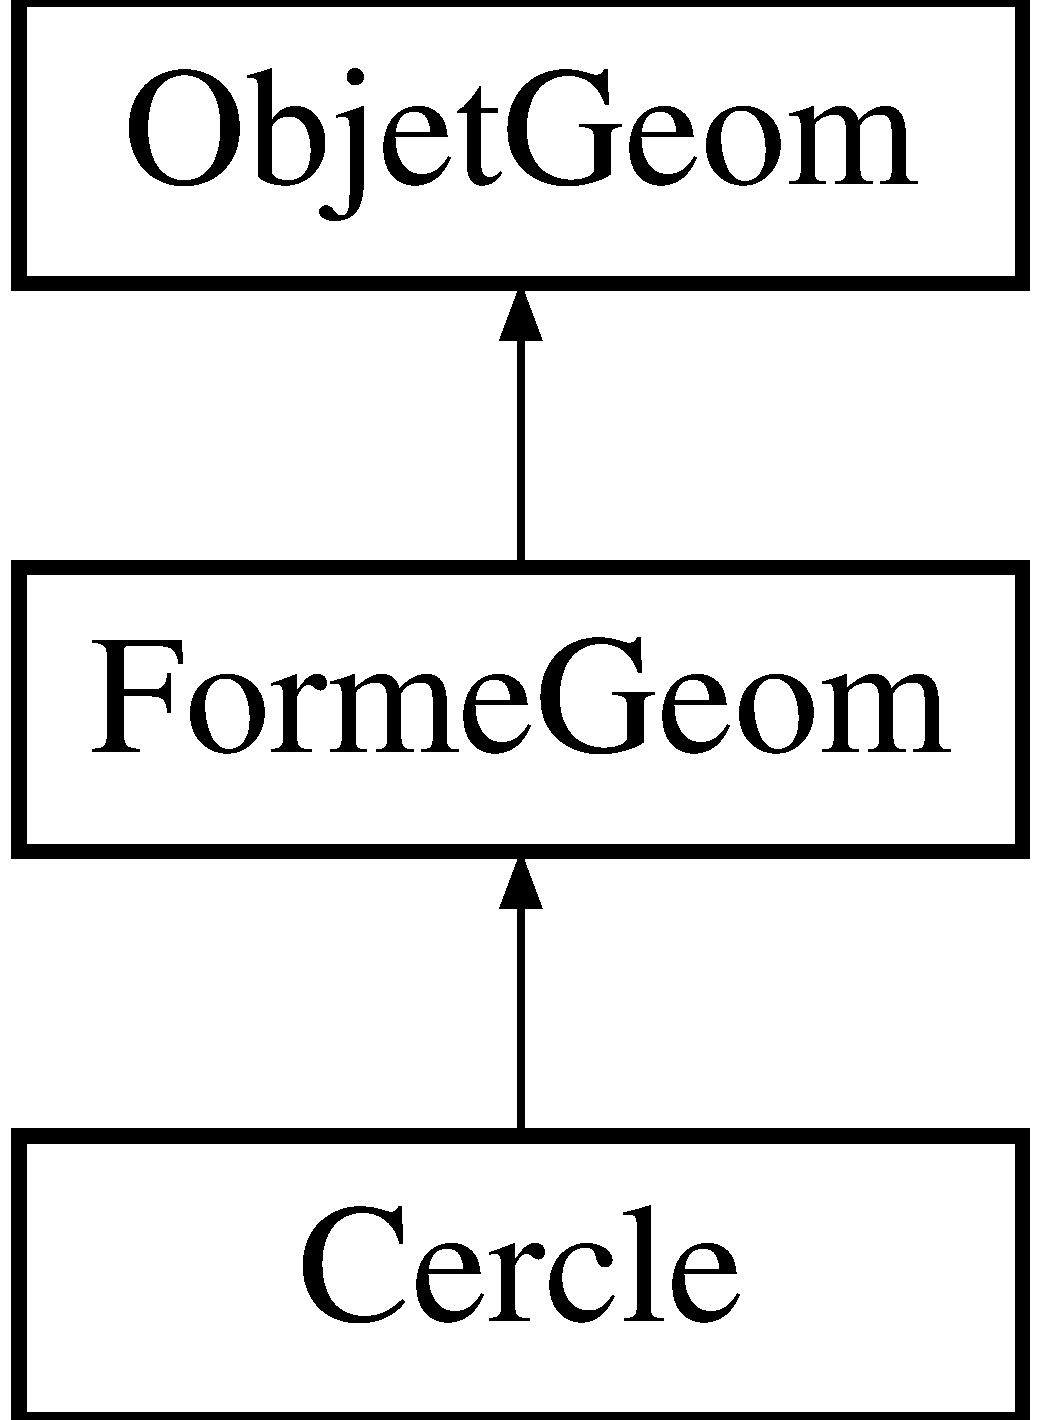
\includegraphics[height=3.000000cm]{class_cercle}
\end{center}
\end{figure}
\subsection*{Fonctions membres publiques}
\begin{DoxyCompactItemize}
\item 
\hypertarget{class_cercle_a3d45994e39b3b024cba60948f18e703e}{{\bfseries Cercle} (const \hyperlink{class_point}{Point} \&centre, double rayon)}\label{class_cercle_a3d45994e39b3b024cba60948f18e703e}

\item 
\hypertarget{class_cercle_ae152ca9e95f7da6c815ddef741eff8b0}{{\bfseries Cercle} (const Couleurs\+::\+Couleur \&couleur, const \hyperlink{class_point}{Point} \&centre, double rayon)}\label{class_cercle_ae152ca9e95f7da6c815ddef741eff8b0}

\item 
\hypertarget{class_cercle_ad107d1ad2b6e5e892fcb70d82f36ebdb}{\hyperlink{class_point}{Point} {\bfseries get\+Centre} () const }\label{class_cercle_ad107d1ad2b6e5e892fcb70d82f36ebdb}

\item 
\hypertarget{class_cercle_ad3ef93ca7d0f9fd73b888f1be9de3e88}{double {\bfseries get\+Rayon} () const }\label{class_cercle_ad3ef93ca7d0f9fd73b888f1be9de3e88}

\item 
\hypertarget{class_cercle_ab9c48b73db7a8467dea0200345ad1174}{virtual \hyperlink{class_cercle}{Cercle} $\ast$ {\bfseries rotation} (const \hyperlink{class_point}{Point} \&p, const \hyperlink{class_angle}{Angle} \&angle) const }\label{class_cercle_ab9c48b73db7a8467dea0200345ad1174}

\item 
\hypertarget{class_cercle_a631711475656f1ea3ceb4d7b035f008c}{virtual \hyperlink{class_cercle}{Cercle} $\ast$ {\bfseries homothetie} (const \hyperlink{class_point}{Point} \&p, const double \&scale) const }\label{class_cercle_a631711475656f1ea3ceb4d7b035f008c}

\item 
\hypertarget{class_cercle_a2cf96d253541d90b990672adbe6ef255}{virtual \hyperlink{class_cercle}{Cercle} $\ast$ {\bfseries translation} (const \hyperlink{class_vecteur}{Vecteur} \&v) const }\label{class_cercle_a2cf96d253541d90b990672adbe6ef255}

\item 
\hypertarget{class_cercle_a306c2e253da2f7c22b6fb17f9888941f}{virtual string {\bfseries to\+String} () const }\label{class_cercle_a306c2e253da2f7c22b6fb17f9888941f}

\item 
\hypertarget{class_cercle_afc10e82bdd08d4c2a1e15265041cf1d9}{virtual double {\bfseries aire} () const }\label{class_cercle_afc10e82bdd08d4c2a1e15265041cf1d9}

\item 
\hypertarget{class_cercle_a4161496710fd6dadf29dcc0361e445e2}{virtual void {\bfseries dessin} (const \hyperlink{class_dessinable}{Dessinable} \&) const }\label{class_cercle_a4161496710fd6dadf29dcc0361e445e2}

\item 
\hypertarget{class_cercle_a13a9c4f9b5fe1485b3ea74a829a82b22}{virtual \hyperlink{class_cercle}{Cercle} $\ast$ {\bfseries clone} () const }\label{class_cercle_a13a9c4f9b5fe1485b3ea74a829a82b22}

\end{DoxyCompactItemize}
\subsection*{Membres hérités additionnels}


\subsection{Description détaillée}
The \hyperlink{class_cercle}{Cercle} class Cette classe représente un cercle, c'est à dire un point pour le centre et un double représentant le rayon. 

La documentation de cette classe a été générée à partir des fichiers suivants \+:\begin{DoxyCompactItemize}
\item 
cercle.\+h\item 
cercle.\+cpp\end{DoxyCompactItemize}

\hypertarget{class_chargement_cercle}{\section{Référence de la classe Chargement\+Cercle}
\label{class_chargement_cercle}\index{Chargement\+Cercle@{Chargement\+Cercle}}
}
Graphe d'héritage de Chargement\+Cercle\+:\begin{figure}[H]
\begin{center}
\leavevmode
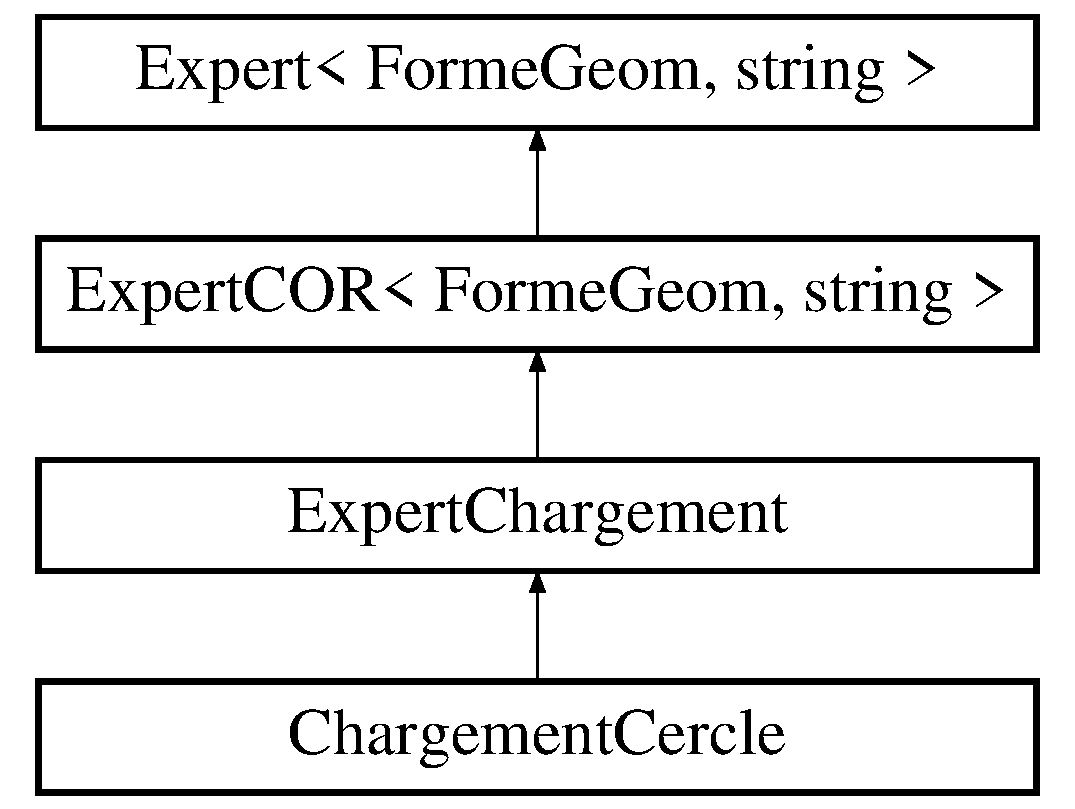
\includegraphics[height=4.000000cm]{class_chargement_cercle}
\end{center}
\end{figure}
\subsection*{Fonctions membres publiques}
\begin{DoxyCompactItemize}
\item 
virtual \hyperlink{class_cercle}{Cercle} $\ast$ \hyperlink{class_chargement_cercle_addd0be00b764eb7736aac2386bbafabd}{traitement\+Specialise} (string \&objet) const 
\begin{DoxyCompactList}\small\item\em traitement1 \end{DoxyCompactList}\end{DoxyCompactItemize}


\subsection{Documentation des fonctions membres}
\hypertarget{class_chargement_cercle_addd0be00b764eb7736aac2386bbafabd}{\index{Chargement\+Cercle@{Chargement\+Cercle}!traitement\+Specialise@{traitement\+Specialise}}
\index{traitement\+Specialise@{traitement\+Specialise}!Chargement\+Cercle@{Chargement\+Cercle}}
\subsubsection[{traitement\+Specialise}]{\setlength{\rightskip}{0pt plus 5cm}virtual {\bf Cercle}$\ast$ Chargement\+Cercle\+::traitement\+Specialise (
\begin{DoxyParamCaption}
\item[{string \&}]{objet}
\end{DoxyParamCaption}
) const\hspace{0.3cm}{\ttfamily [inline]}, {\ttfamily [virtual]}}}\label{class_chargement_cercle_addd0be00b764eb7736aac2386bbafabd}


traitement1 


\begin{DoxyParams}{Paramètres}
{\em objet} & \\
\hline
\end{DoxyParams}
\begin{DoxyReturn}{Renvoie}
l'objet parsé ou N\+U\+L\+L si non trouvé. 
\end{DoxyReturn}


Implémente \hyperlink{class_expert_chargement_a7d7818bdd5f0a06b06bfc8047ec8fee5}{Expert\+Chargement}.



La documentation de cette classe a été générée à partir du fichier suivant \+:\begin{DoxyCompactItemize}
\item 
chargement\+C\+O\+R/chargementcercle.\+h\end{DoxyCompactItemize}

\hypertarget{class_chargement_facade}{\section{Référence de la classe Chargement\+Facade}
\label{class_chargement_facade}\index{Chargement\+Facade@{Chargement\+Facade}}
}
Graphe d'héritage de Chargement\+Facade\+:\begin{figure}[H]
\begin{center}
\leavevmode
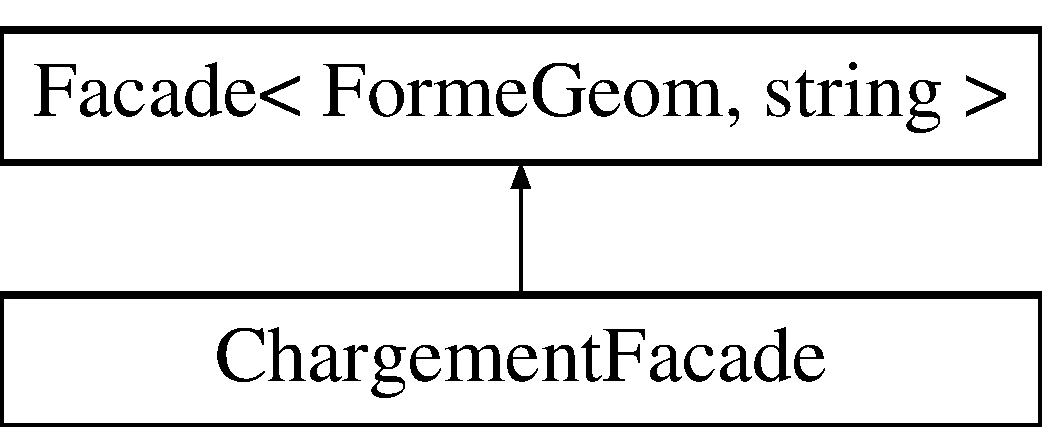
\includegraphics[height=2.000000cm]{class_chargement_facade}
\end{center}
\end{figure}
\subsection*{Fonctions membres publiques}
\begin{DoxyCompactItemize}
\item 
\hypertarget{class_chargement_facade_a11b9b3e10e86363a11ac00474ef41a68}{{\bfseries Chargement\+Facade} (ifstream \&file)}\label{class_chargement_facade_a11b9b3e10e86363a11ac00474ef41a68}

\item 
\hypertarget{class_chargement_facade_aaabf98f68708f461ce8d98a42c2b6b59}{{\bfseries Chargement\+Facade} (string contenu)}\label{class_chargement_facade_aaabf98f68708f461ce8d98a42c2b6b59}

\end{DoxyCompactItemize}
\subsection*{Membres hérités additionnels}


La documentation de cette classe a été générée à partir du fichier suivant \+:\begin{DoxyCompactItemize}
\item 
chargement\+C\+O\+R/chargementfacade.\+h\end{DoxyCompactItemize}

\hypertarget{class_chargement_groupe}{\section{Référence de la classe Chargement\+Groupe}
\label{class_chargement_groupe}\index{Chargement\+Groupe@{Chargement\+Groupe}}
}
Graphe d'héritage de Chargement\+Groupe\+:\begin{figure}[H]
\begin{center}
\leavevmode
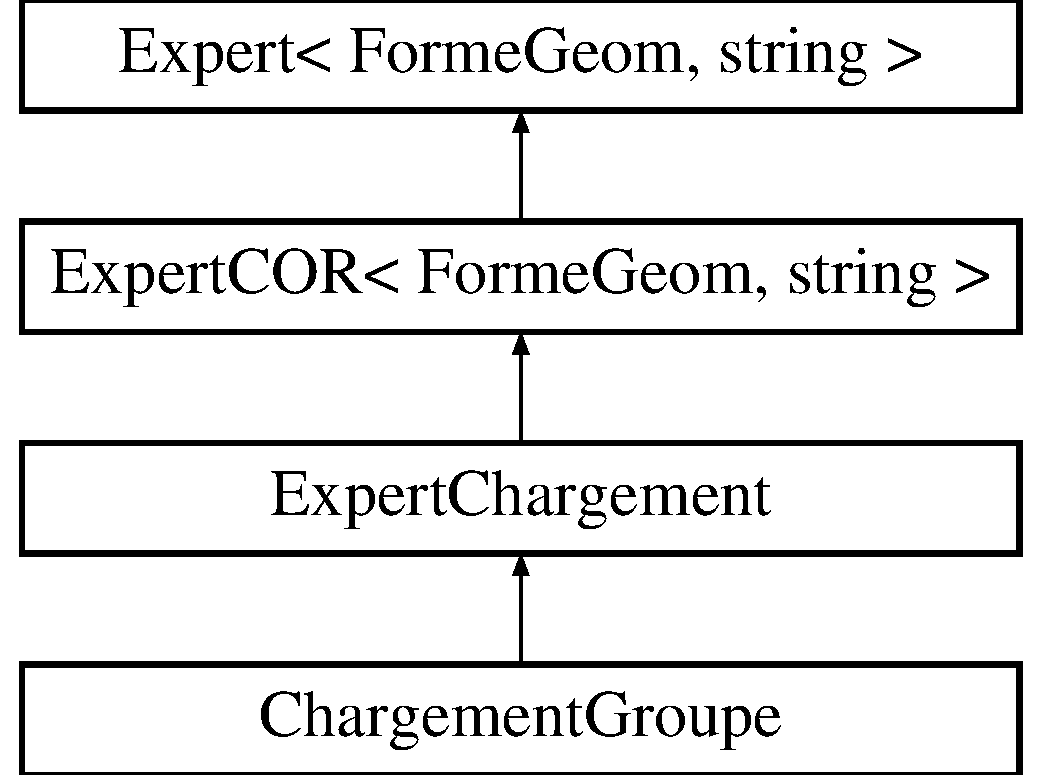
\includegraphics[height=4.000000cm]{class_chargement_groupe}
\end{center}
\end{figure}
\subsection*{Fonctions membres publiques}
\begin{DoxyCompactItemize}
\item 
virtual \hyperlink{class_groupe}{Groupe} $\ast$ \hyperlink{class_chargement_groupe_aa0487a2d01a2c8022fbaf854e79bafd6}{traitement\+Specialise} (string \&objet) const 
\begin{DoxyCompactList}\small\item\em traitement1 \end{DoxyCompactList}\end{DoxyCompactItemize}


\subsection{Documentation des fonctions membres}
\hypertarget{class_chargement_groupe_aa0487a2d01a2c8022fbaf854e79bafd6}{\index{Chargement\+Groupe@{Chargement\+Groupe}!traitement\+Specialise@{traitement\+Specialise}}
\index{traitement\+Specialise@{traitement\+Specialise}!Chargement\+Groupe@{Chargement\+Groupe}}
\subsubsection[{traitement\+Specialise}]{\setlength{\rightskip}{0pt plus 5cm}{\bf Groupe} $\ast$ Chargement\+Groupe\+::traitement\+Specialise (
\begin{DoxyParamCaption}
\item[{string \&}]{objet}
\end{DoxyParamCaption}
) const\hspace{0.3cm}{\ttfamily [virtual]}}}\label{class_chargement_groupe_aa0487a2d01a2c8022fbaf854e79bafd6}


traitement1 


\begin{DoxyParams}{Paramètres}
{\em objet} & \\
\hline
\end{DoxyParams}
\begin{DoxyReturn}{Renvoie}
l'objet parsé ou N\+U\+L\+L si non trouvé. 
\end{DoxyReturn}


Implémente \hyperlink{class_expert_chargement_a7d7818bdd5f0a06b06bfc8047ec8fee5}{Expert\+Chargement}.



La documentation de cette classe a été générée à partir des fichiers suivants \+:\begin{DoxyCompactItemize}
\item 
chargement\+C\+O\+R/chargementgroupe.\+h\item 
chargement\+C\+O\+R/chargementgroupe.\+cpp\end{DoxyCompactItemize}

\hypertarget{class_chargement_polygone}{\section{Référence de la classe Chargement\+Polygone}
\label{class_chargement_polygone}\index{Chargement\+Polygone@{Chargement\+Polygone}}
}
Graphe d'héritage de Chargement\+Polygone\+:\begin{figure}[H]
\begin{center}
\leavevmode
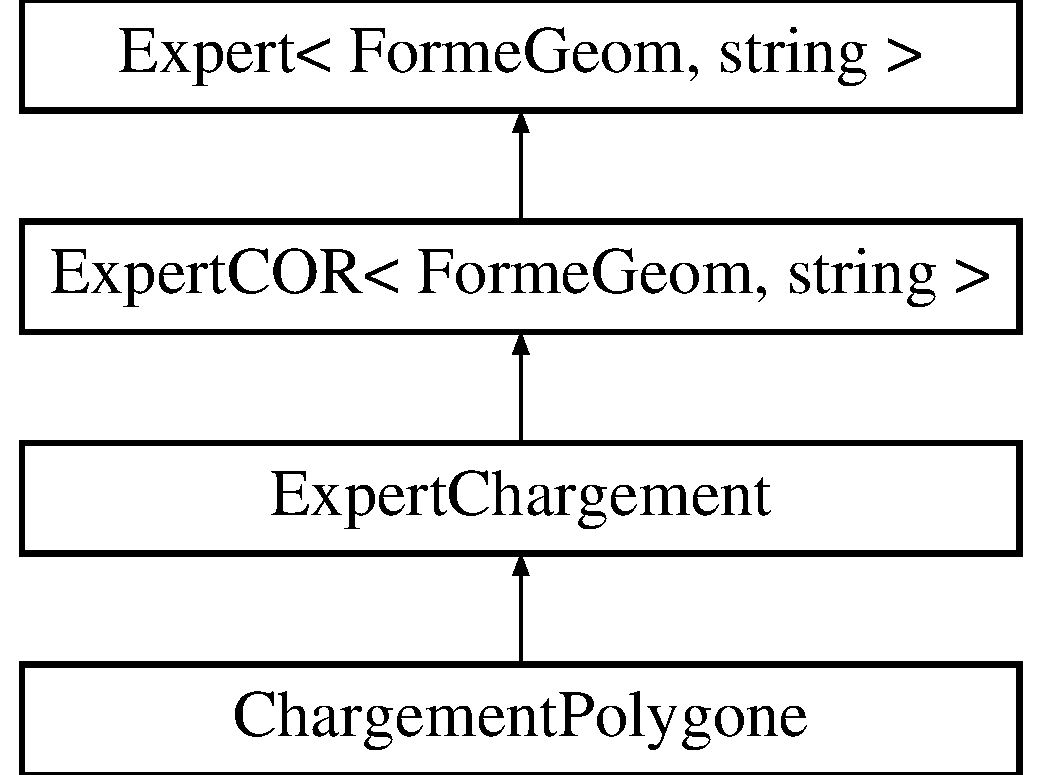
\includegraphics[height=4.000000cm]{class_chargement_polygone}
\end{center}
\end{figure}
\subsection*{Fonctions membres publiques}
\begin{DoxyCompactItemize}
\item 
virtual \hyperlink{class_polygone}{Polygone} $\ast$ \hyperlink{class_chargement_polygone_a66c85c1a8a6aba246a283aaa18bfddd4}{traitement\+Specialise} (string \&objet) const 
\begin{DoxyCompactList}\small\item\em traitement1 \end{DoxyCompactList}\end{DoxyCompactItemize}


\subsection{Documentation des fonctions membres}
\hypertarget{class_chargement_polygone_a66c85c1a8a6aba246a283aaa18bfddd4}{\index{Chargement\+Polygone@{Chargement\+Polygone}!traitement\+Specialise@{traitement\+Specialise}}
\index{traitement\+Specialise@{traitement\+Specialise}!Chargement\+Polygone@{Chargement\+Polygone}}
\subsubsection[{traitement\+Specialise}]{\setlength{\rightskip}{0pt plus 5cm}virtual {\bf Polygone}$\ast$ Chargement\+Polygone\+::traitement\+Specialise (
\begin{DoxyParamCaption}
\item[{string \&}]{objet}
\end{DoxyParamCaption}
) const\hspace{0.3cm}{\ttfamily [inline]}, {\ttfamily [virtual]}}}\label{class_chargement_polygone_a66c85c1a8a6aba246a283aaa18bfddd4}


traitement1 


\begin{DoxyParams}{Paramètres}
{\em objet} & \\
\hline
\end{DoxyParams}
\begin{DoxyReturn}{Renvoie}
l'objet parsé ou N\+U\+L\+L si non trouvé. 
\end{DoxyReturn}


Implémente \hyperlink{class_expert_chargement_a7d7818bdd5f0a06b06bfc8047ec8fee5}{Expert\+Chargement}.



La documentation de cette classe a été générée à partir du fichier suivant \+:\begin{DoxyCompactItemize}
\item 
chargement\+C\+O\+R/chargementpolygone.\+h\end{DoxyCompactItemize}

\hypertarget{class_chargement_segment}{\section{Référence de la classe Chargement\+Segment}
\label{class_chargement_segment}\index{Chargement\+Segment@{Chargement\+Segment}}
}
Graphe d'héritage de Chargement\+Segment\+:\begin{figure}[H]
\begin{center}
\leavevmode
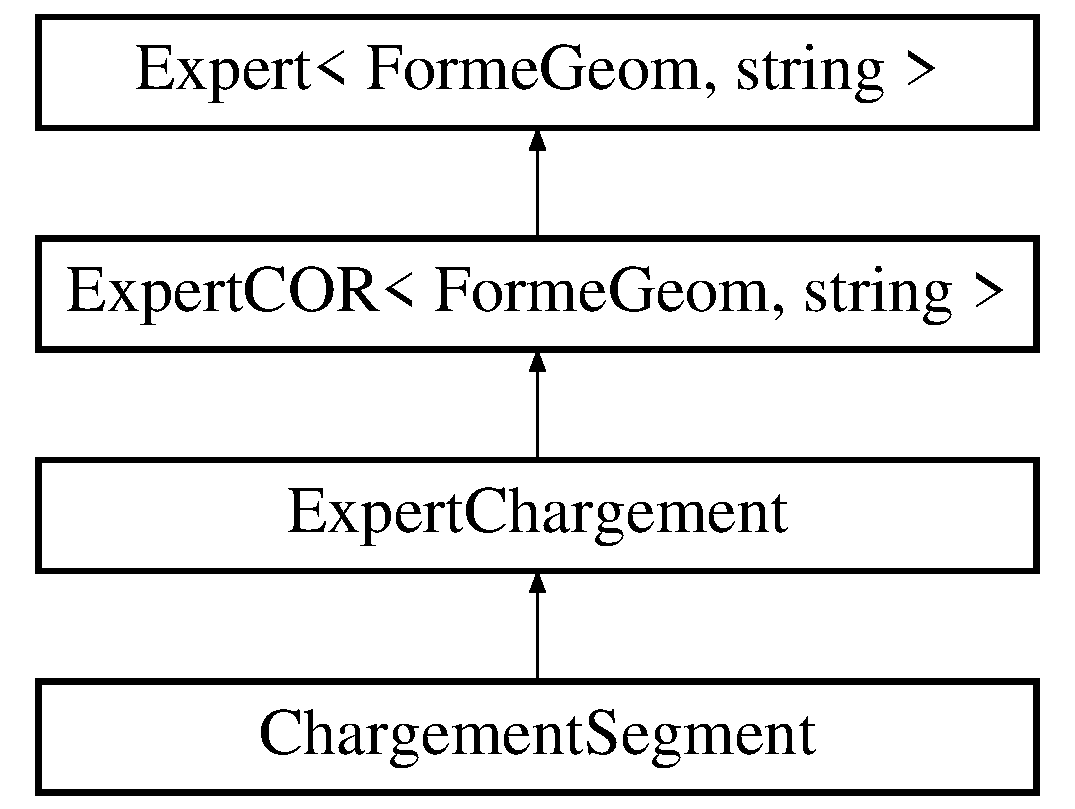
\includegraphics[height=4.000000cm]{class_chargement_segment}
\end{center}
\end{figure}
\subsection*{Fonctions membres publiques}
\begin{DoxyCompactItemize}
\item 
virtual \hyperlink{class_segment}{Segment} $\ast$ \hyperlink{class_chargement_segment_ab03da7e3e7870d2522d72095ae827135}{traitement\+Specialise} (string \&objet) const 
\begin{DoxyCompactList}\small\item\em traitement1 \end{DoxyCompactList}\end{DoxyCompactItemize}


\subsection{Documentation des fonctions membres}
\hypertarget{class_chargement_segment_ab03da7e3e7870d2522d72095ae827135}{\index{Chargement\+Segment@{Chargement\+Segment}!traitement\+Specialise@{traitement\+Specialise}}
\index{traitement\+Specialise@{traitement\+Specialise}!Chargement\+Segment@{Chargement\+Segment}}
\subsubsection[{traitement\+Specialise}]{\setlength{\rightskip}{0pt plus 5cm}virtual {\bf Segment}$\ast$ Chargement\+Segment\+::traitement\+Specialise (
\begin{DoxyParamCaption}
\item[{string \&}]{objet}
\end{DoxyParamCaption}
) const\hspace{0.3cm}{\ttfamily [inline]}, {\ttfamily [virtual]}}}\label{class_chargement_segment_ab03da7e3e7870d2522d72095ae827135}


traitement1 


\begin{DoxyParams}{Paramètres}
{\em objet} & \\
\hline
\end{DoxyParams}
\begin{DoxyReturn}{Renvoie}
l'objet parsé ou N\+U\+L\+L si non trouvé. 
\end{DoxyReturn}


Implémente \hyperlink{class_expert_chargement_a7d7818bdd5f0a06b06bfc8047ec8fee5}{Expert\+Chargement}.



La documentation de cette classe a été générée à partir du fichier suivant \+:\begin{DoxyCompactItemize}
\item 
chargement\+C\+O\+R/chargementsegment.\+h\end{DoxyCompactItemize}

\hypertarget{class_chargement_triangle}{\section{Référence de la classe Chargement\+Triangle}
\label{class_chargement_triangle}\index{Chargement\+Triangle@{Chargement\+Triangle}}
}
Graphe d'héritage de Chargement\+Triangle\+:\begin{figure}[H]
\begin{center}
\leavevmode
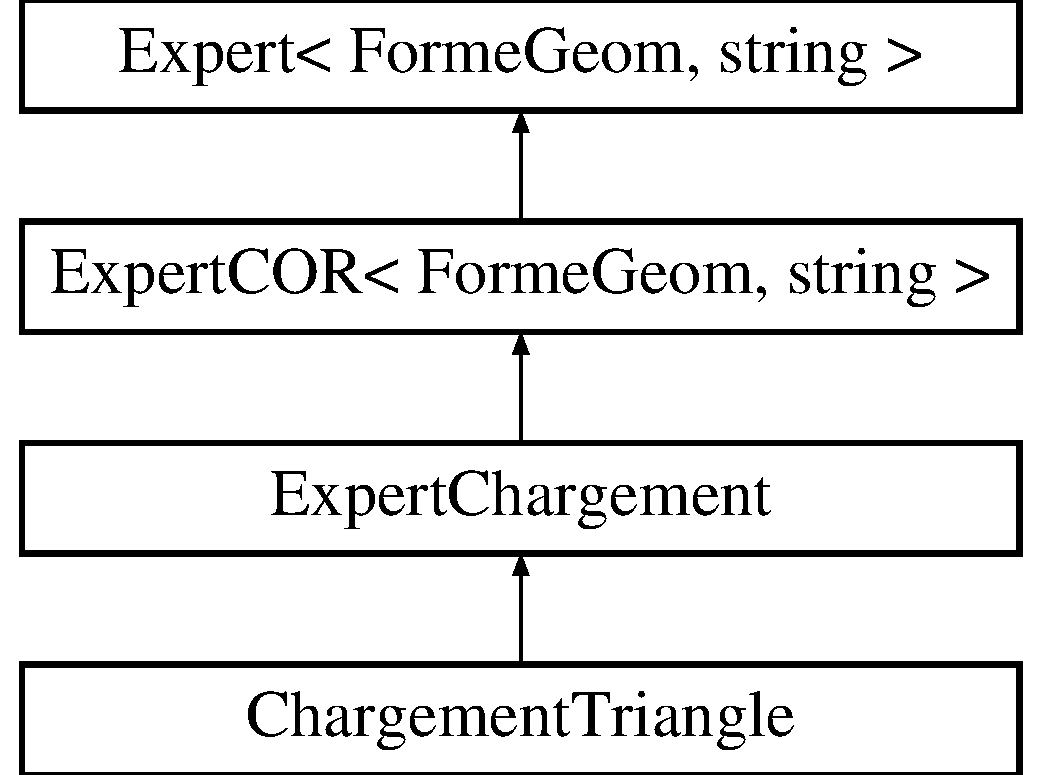
\includegraphics[height=4.000000cm]{class_chargement_triangle}
\end{center}
\end{figure}
\subsection*{Fonctions membres publiques}
\begin{DoxyCompactItemize}
\item 
virtual \hyperlink{class_triangle}{Triangle} $\ast$ \hyperlink{class_chargement_triangle_a5a56b270c58404c940900c5d93237876}{traitement\+Specialise} (string \&objet) const 
\begin{DoxyCompactList}\small\item\em traitement1 \end{DoxyCompactList}\end{DoxyCompactItemize}


\subsection{Documentation des fonctions membres}
\hypertarget{class_chargement_triangle_a5a56b270c58404c940900c5d93237876}{\index{Chargement\+Triangle@{Chargement\+Triangle}!traitement\+Specialise@{traitement\+Specialise}}
\index{traitement\+Specialise@{traitement\+Specialise}!Chargement\+Triangle@{Chargement\+Triangle}}
\subsubsection[{traitement\+Specialise}]{\setlength{\rightskip}{0pt plus 5cm}virtual {\bf Triangle}$\ast$ Chargement\+Triangle\+::traitement\+Specialise (
\begin{DoxyParamCaption}
\item[{string \&}]{objet}
\end{DoxyParamCaption}
) const\hspace{0.3cm}{\ttfamily [inline]}, {\ttfamily [virtual]}}}\label{class_chargement_triangle_a5a56b270c58404c940900c5d93237876}


traitement1 


\begin{DoxyParams}{Paramètres}
{\em objet} & \\
\hline
\end{DoxyParams}
\begin{DoxyReturn}{Renvoie}
l'objet parsé ou N\+U\+L\+L si non trouvé. 
\end{DoxyReturn}


Implémente \hyperlink{class_expert_chargement_a7d7818bdd5f0a06b06bfc8047ec8fee5}{Expert\+Chargement}.



La documentation de cette classe a été générée à partir du fichier suivant \+:\begin{DoxyCompactItemize}
\item 
chargement\+C\+O\+R/chargementtriangle.\+h\end{DoxyCompactItemize}

\hypertarget{class_connexion}{\section{Référence de la classe Connexion}
\label{class_connexion}\index{Connexion@{Connexion}}
}


The \hyperlink{class_connexion}{Connexion} class Cette classe est charg�e d'�tablire une connexion avec un serveur distant Cette classe charge une seule fois les dll Windows pour toutes les instances, cette partie est donc un singleton. De plus elle est compilable et fonctionnelle sous windows et unix(linux / mac compris) car la portabilit� c'est la vie.  




{\ttfamily \#include $<$connexion.\+h$>$}

\subsection*{Fonctions membres publiques}
\begin{DoxyCompactItemize}
\item 
\hypertarget{class_connexion_a7c890dbf77a2b9f49013a7be018d2230}{{\bfseries Connexion} (const std\+::string \&ip, int host)}\label{class_connexion_a7c890dbf77a2b9f49013a7be018d2230}

\item 
void \hyperlink{class_connexion_aa8fbcb5c7ae95474159841a159075d72}{envoyer} (const char $\ast$) const 
\begin{DoxyCompactList}\small\item\em \hyperlink{class_connexion_aa8fbcb5c7ae95474159841a159075d72}{Connexion\+::envoyer} envoie le message au serveur. \end{DoxyCompactList}\item 
int \hyperlink{class_connexion_aff85c238e81fb5e3b7b5e218da2b70ef}{recevoir} () const 
\begin{DoxyCompactList}\small\item\em Dessin\+Manager\+::recevoir. \end{DoxyCompactList}\end{DoxyCompactItemize}


\subsection{Description détaillée}
The \hyperlink{class_connexion}{Connexion} class Cette classe est charg�e d'�tablire une connexion avec un serveur distant Cette classe charge une seule fois les dll Windows pour toutes les instances, cette partie est donc un singleton. De plus elle est compilable et fonctionnelle sous windows et unix(linux / mac compris) car la portabilit� c'est la vie. 

\subsection{Documentation des fonctions membres}
\hypertarget{class_connexion_aa8fbcb5c7ae95474159841a159075d72}{\index{Connexion@{Connexion}!envoyer@{envoyer}}
\index{envoyer@{envoyer}!Connexion@{Connexion}}
\subsubsection[{envoyer}]{\setlength{\rightskip}{0pt plus 5cm}void Connexion\+::envoyer (
\begin{DoxyParamCaption}
\item[{const char $\ast$}]{message}
\end{DoxyParamCaption}
) const}}\label{class_connexion_aa8fbcb5c7ae95474159841a159075d72}


\hyperlink{class_connexion_aa8fbcb5c7ae95474159841a159075d72}{Connexion\+::envoyer} envoie le message au serveur. 


\begin{DoxyParams}{Paramètres}
{\em message} & le message � envoyer Cette m�thode permet d'envoyer un message au serveur Il ne faut pas ajouter \char`\"{}\textbackslash{}r\textbackslash{}n\char`\"{} � la fin du message, la fonction s'en charge. \\
\hline
\end{DoxyParams}
\hypertarget{class_connexion_aff85c238e81fb5e3b7b5e218da2b70ef}{\index{Connexion@{Connexion}!recevoir@{recevoir}}
\index{recevoir@{recevoir}!Connexion@{Connexion}}
\subsubsection[{recevoir}]{\setlength{\rightskip}{0pt plus 5cm}int Connexion\+::recevoir (
\begin{DoxyParamCaption}
{}
\end{DoxyParamCaption}
) const}}\label{class_connexion_aff85c238e81fb5e3b7b5e218da2b70ef}


Dessin\+Manager\+::recevoir. 

\begin{DoxyReturn}{Renvoie}
la r�ponse du serveur, 0 (il y a eu une erreur) ou 1 (tout s'est bien pass�) Fonction � appeller apr�s chaque envoie de message, elle v�rifie que le message a bien �t� re�u par le serveur 
\end{DoxyReturn}


La documentation de cette classe a été générée à partir des fichiers suivants \+:\begin{DoxyCompactItemize}
\item 
connexion.\+h\item 
connexion.\+cpp\end{DoxyCompactItemize}

\hypertarget{class_couleurs}{\section{Référence de la classe Couleurs}
\label{class_couleurs}\index{Couleurs@{Couleurs}}
}


The \hyperlink{class_couleurs}{Couleurs} class Cette classe représente les différentes couleurs disponible dans l'application et contient les différentes méthodes utiles pour les manipuler.  




{\ttfamily \#include $<$Couleur.\+h$>$}

\subsection*{Types publics}
\begin{DoxyCompactItemize}
\item 
\hypertarget{class_couleurs_abd168094c41895357f4402e17bcd7379}{enum {\bfseries Couleur} \{ \\*
{\bfseries black} = 0, 
{\bfseries white}, 
{\bfseries yellow}, 
{\bfseries red}, 
\\*
{\bfseries green}, 
{\bfseries blue}, 
{\bfseries nb\+Couleurs}
 \}}\label{class_couleurs_abd168094c41895357f4402e17bcd7379}

\end{DoxyCompactItemize}
\subsection*{Fonctions membres publiques statiques}
\begin{DoxyCompactItemize}
\item 
static string \hyperlink{class_couleurs_a3a07aadeec400f7ae9aa2f7548732609}{couleur\+To\+String} (const Couleur \&couleur)
\begin{DoxyCompactList}\small\item\em couleur\+To\+String \end{DoxyCompactList}\item 
static string \hyperlink{class_couleurs_a180a77b65f68f5bfa07c7bf0755cced8}{couleur\+To\+Hexa} (const Couleur \&couleur)
\begin{DoxyCompactList}\small\item\em couleur\+To\+Hexa \end{DoxyCompactList}\item 
static Couleur \hyperlink{class_couleurs_a502cfe3fdf9496d4b2f391d68b3ec00f}{hexa\+To\+Couleur} (const string \&hexa)
\begin{DoxyCompactList}\small\item\em hexa\+To\+Couleur \end{DoxyCompactList}\item 
static Couleur \hyperlink{class_couleurs_a4c1d1a7dad74a2337920103313c7ddbc}{string\+To\+Couleur} (const string \&nom)
\begin{DoxyCompactList}\small\item\em string\+To\+Couleur \end{DoxyCompactList}\item 
static Couleur \hyperlink{class_couleurs_ade385a32c027d77eef94fff699e23ac4}{int\+To\+Couleur} (int i)
\begin{DoxyCompactList}\small\item\em int\+To\+Couleur \end{DoxyCompactList}\item 
static bool \hyperlink{class_couleurs_aa9b1467aaf1b88acbefc3e319a9a32bf}{is\+Couleur} (const string \&coul)
\begin{DoxyCompactList}\small\item\em is\+Couleur \end{DoxyCompactList}\end{DoxyCompactItemize}
\subsection*{Amis}
\begin{DoxyCompactItemize}
\item 
\hypertarget{class_couleurs_acad36b0faad1100a0bf903291f8506db}{ostream \& {\bfseries operator$<$$<$} (ostream \&, const Couleur \&c)}\label{class_couleurs_acad36b0faad1100a0bf903291f8506db}

\end{DoxyCompactItemize}


\subsection{Description détaillée}
The \hyperlink{class_couleurs}{Couleurs} class Cette classe représente les différentes couleurs disponible dans l'application et contient les différentes méthodes utiles pour les manipuler. 

\subsection{Documentation des fonctions membres}
\hypertarget{class_couleurs_a180a77b65f68f5bfa07c7bf0755cced8}{\index{Couleurs@{Couleurs}!couleur\+To\+Hexa@{couleur\+To\+Hexa}}
\index{couleur\+To\+Hexa@{couleur\+To\+Hexa}!Couleurs@{Couleurs}}
\subsubsection[{couleur\+To\+Hexa}]{\setlength{\rightskip}{0pt plus 5cm}string Couleurs\+::couleur\+To\+Hexa (
\begin{DoxyParamCaption}
\item[{const Couleur \&}]{couleur}
\end{DoxyParamCaption}
)\hspace{0.3cm}{\ttfamily [static]}}}\label{class_couleurs_a180a77b65f68f5bfa07c7bf0755cced8}


couleur\+To\+Hexa 

couleur\+To\+Hexa Permet d'obtenir le code hexadécimal correspondant à une couleur


\begin{DoxyParams}{Paramètres}
{\em couleur} & \\
\hline
\end{DoxyParams}
\begin{DoxyReturn}{Renvoie}
un string représentant la valeur hexadécimale de la couleur passée en paramètre sous la forme\+: \char`\"{}\#\+R\+R\+G\+G\+B\+B\char`\"{}.
\end{DoxyReturn}

\begin{DoxyParams}{Paramètres}
{\em couleur} & \\
\hline
\end{DoxyParams}
\begin{DoxyReturn}{Renvoie}
le code hexadeciale sous la forme \char`\"{}\#\+R\+R\+G\+G\+B\+B\char`\"{} 
\end{DoxyReturn}
\hypertarget{class_couleurs_a3a07aadeec400f7ae9aa2f7548732609}{\index{Couleurs@{Couleurs}!couleur\+To\+String@{couleur\+To\+String}}
\index{couleur\+To\+String@{couleur\+To\+String}!Couleurs@{Couleurs}}
\subsubsection[{couleur\+To\+String}]{\setlength{\rightskip}{0pt plus 5cm}string Couleurs\+::couleur\+To\+String (
\begin{DoxyParamCaption}
\item[{const Couleur \&}]{couleur}
\end{DoxyParamCaption}
)\hspace{0.3cm}{\ttfamily [static]}}}\label{class_couleurs_a3a07aadeec400f7ae9aa2f7548732609}


couleur\+To\+String 


\begin{DoxyParams}{Paramètres}
{\em couleur} & \\
\hline
\end{DoxyParams}
\begin{DoxyReturn}{Renvoie}
un string représentant la couleur passée en paramètre 
\end{DoxyReturn}
\hypertarget{class_couleurs_a502cfe3fdf9496d4b2f391d68b3ec00f}{\index{Couleurs@{Couleurs}!hexa\+To\+Couleur@{hexa\+To\+Couleur}}
\index{hexa\+To\+Couleur@{hexa\+To\+Couleur}!Couleurs@{Couleurs}}
\subsubsection[{hexa\+To\+Couleur}]{\setlength{\rightskip}{0pt plus 5cm}Couleurs\+::\+Couleur Couleurs\+::hexa\+To\+Couleur (
\begin{DoxyParamCaption}
\item[{const string \&}]{hexa}
\end{DoxyParamCaption}
)\hspace{0.3cm}{\ttfamily [static]}}}\label{class_couleurs_a502cfe3fdf9496d4b2f391d68b3ec00f}


hexa\+To\+Couleur 


\begin{DoxyParams}{Paramètres}
{\em hexa} & \\
\hline
\end{DoxyParams}
\begin{DoxyReturn}{Renvoie}
la couleur correspondant à la valeur hexadécimale passée en paramètre. Retourne Couleur\+::nb\+Couleurs si la couleur n'est pas trouvée. 
\end{DoxyReturn}
\hypertarget{class_couleurs_ade385a32c027d77eef94fff699e23ac4}{\index{Couleurs@{Couleurs}!int\+To\+Couleur@{int\+To\+Couleur}}
\index{int\+To\+Couleur@{int\+To\+Couleur}!Couleurs@{Couleurs}}
\subsubsection[{int\+To\+Couleur}]{\setlength{\rightskip}{0pt plus 5cm}Couleurs\+::\+Couleur Couleurs\+::int\+To\+Couleur (
\begin{DoxyParamCaption}
\item[{int}]{i}
\end{DoxyParamCaption}
)\hspace{0.3cm}{\ttfamily [static]}}}\label{class_couleurs_ade385a32c027d77eef94fff699e23ac4}


int\+To\+Couleur 


\begin{DoxyParams}{Paramètres}
{\em i} & \\
\hline
\end{DoxyParams}
\begin{DoxyReturn}{Renvoie}
la couleur correspondant à l'indice, si l'indice ne correspond à aucune couleur, on retourne Couleurs\+::nb\+Couleurs . 
\end{DoxyReturn}
\hypertarget{class_couleurs_aa9b1467aaf1b88acbefc3e319a9a32bf}{\index{Couleurs@{Couleurs}!is\+Couleur@{is\+Couleur}}
\index{is\+Couleur@{is\+Couleur}!Couleurs@{Couleurs}}
\subsubsection[{is\+Couleur}]{\setlength{\rightskip}{0pt plus 5cm}bool Couleurs\+::is\+Couleur (
\begin{DoxyParamCaption}
\item[{const string \&}]{coul}
\end{DoxyParamCaption}
)\hspace{0.3cm}{\ttfamily [static]}}}\label{class_couleurs_aa9b1467aaf1b88acbefc3e319a9a32bf}


is\+Couleur 


\begin{DoxyParams}{Paramètres}
{\em coul} & \\
\hline
\end{DoxyParams}
\begin{DoxyReturn}{Renvoie}
true si coul est une couleur correcte, false sinon. 
\end{DoxyReturn}
\hypertarget{class_couleurs_a4c1d1a7dad74a2337920103313c7ddbc}{\index{Couleurs@{Couleurs}!string\+To\+Couleur@{string\+To\+Couleur}}
\index{string\+To\+Couleur@{string\+To\+Couleur}!Couleurs@{Couleurs}}
\subsubsection[{string\+To\+Couleur}]{\setlength{\rightskip}{0pt plus 5cm}Couleurs\+::\+Couleur Couleurs\+::string\+To\+Couleur (
\begin{DoxyParamCaption}
\item[{const string \&}]{nom}
\end{DoxyParamCaption}
)\hspace{0.3cm}{\ttfamily [static]}}}\label{class_couleurs_a4c1d1a7dad74a2337920103313c7ddbc}


string\+To\+Couleur 


\begin{DoxyParams}{Paramètres}
{\em nom} & \\
\hline
\end{DoxyParams}
\begin{DoxyReturn}{Renvoie}
la couleur correspondant au nom de couleur passé en paramètre. Retourne Couleur\+::nb\+Couleurs si la couleur n'est pas trouvée. 
\end{DoxyReturn}


La documentation de cette classe a été générée à partir des fichiers suivants \+:\begin{DoxyCompactItemize}
\item 
Couleur.\+h\item 
Couleur.\+cpp\end{DoxyCompactItemize}

\hypertarget{class_dessinable}{\section{Référence de la classe Dessinable}
\label{class_dessinable}\index{Dessinable@{Dessinable}}
}


The \hyperlink{class_dessinable}{Dessinable} class Il s'agit d'une interface décrivant le comportement que doivent avoir les classes de dessin. Cette classe sers donc majoritairement à assurer l'évolutivité de l'application en indiquant aux autres classes voulant dessiner les formes géometriques quelles méthodes elles doivent implémenter.  




{\ttfamily \#include $<$dessinable.\+h$>$}

Graphe d'héritage de Dessinable\+:\begin{figure}[H]
\begin{center}
\leavevmode
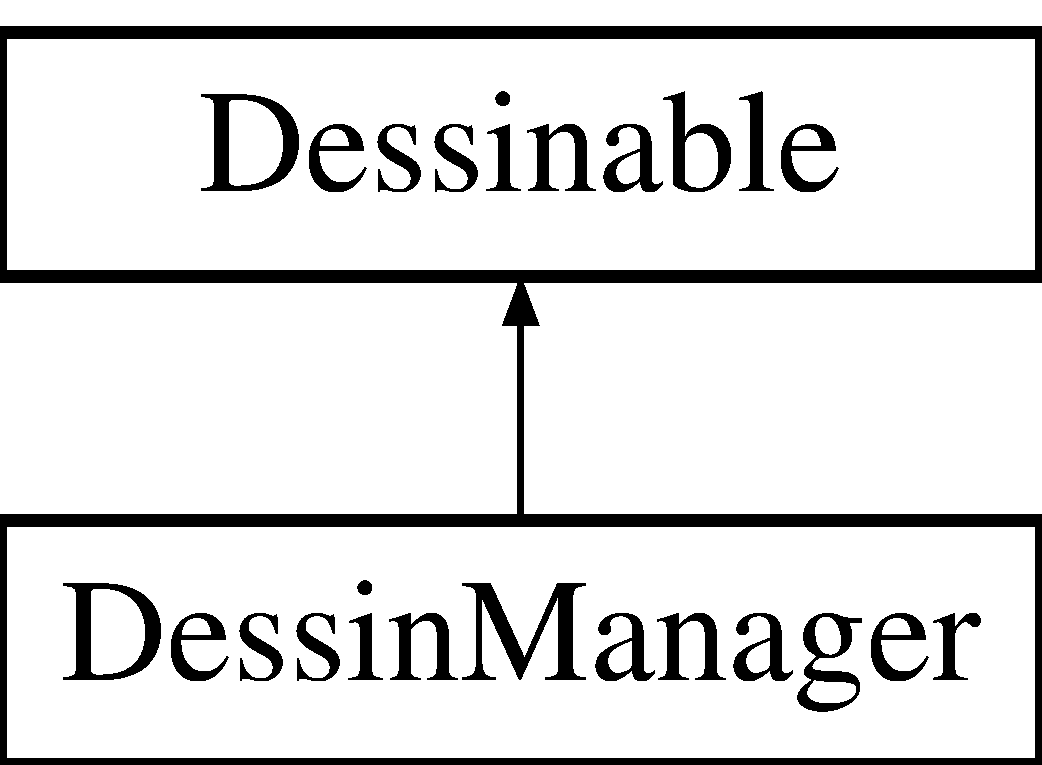
\includegraphics[height=2.000000cm]{class_dessinable}
\end{center}
\end{figure}
\subsection*{Fonctions membres publiques}
\begin{DoxyCompactItemize}
\item 
\hypertarget{class_dessinable_a51d58a1596d60bdb8a4c0f45578031a5}{virtual void {\bfseries dessiner\+Cercle} (const \hyperlink{class_cercle}{Cercle} \&c) const =0}\label{class_dessinable_a51d58a1596d60bdb8a4c0f45578031a5}

\item 
\hypertarget{class_dessinable_a730da0dc2d1d4ec2d967641f4da0c9a8}{virtual void {\bfseries dessiner\+Triangle} (const \hyperlink{class_triangle}{Triangle} \&t) const =0}\label{class_dessinable_a730da0dc2d1d4ec2d967641f4da0c9a8}

\item 
\hypertarget{class_dessinable_a6afb4c5e0fd922cbc76c8e37ebc2e76b}{virtual void {\bfseries dessiner\+Segment} (const \hyperlink{class_segment}{Segment} \&s) const =0}\label{class_dessinable_a6afb4c5e0fd922cbc76c8e37ebc2e76b}

\item 
\hypertarget{class_dessinable_ab3c724ac2612e7aaf3bffb0819d2a38b}{virtual void {\bfseries dessiner\+Polygone} (const \hyperlink{class_polygone}{Polygone} \&p) const =0}\label{class_dessinable_ab3c724ac2612e7aaf3bffb0819d2a38b}

\end{DoxyCompactItemize}


\subsection{Description détaillée}
The \hyperlink{class_dessinable}{Dessinable} class Il s'agit d'une interface décrivant le comportement que doivent avoir les classes de dessin. Cette classe sers donc majoritairement à assurer l'évolutivité de l'application en indiquant aux autres classes voulant dessiner les formes géometriques quelles méthodes elles doivent implémenter. 

La documentation de cette classe a été générée à partir du fichier suivant \+:\begin{DoxyCompactItemize}
\item 
dessinable.\+h\end{DoxyCompactItemize}

\hypertarget{class_dessin_manager}{\section{Référence de la classe Dessin\+Manager}
\label{class_dessin_manager}\index{Dessin\+Manager@{Dessin\+Manager}}
}


The \hyperlink{class_dessin_manager}{Dessin\+Manager} class Cette classe est chargé de dessiner les formes géometriques. Le dessin est fait en envoyant les formes géometriques à un serveur distant afin que celui-\/ci dessine.  




{\ttfamily \#include $<$dessin\+Manager.\+h$>$}

Graphe d'héritage de Dessin\+Manager\+:\begin{figure}[H]
\begin{center}
\leavevmode
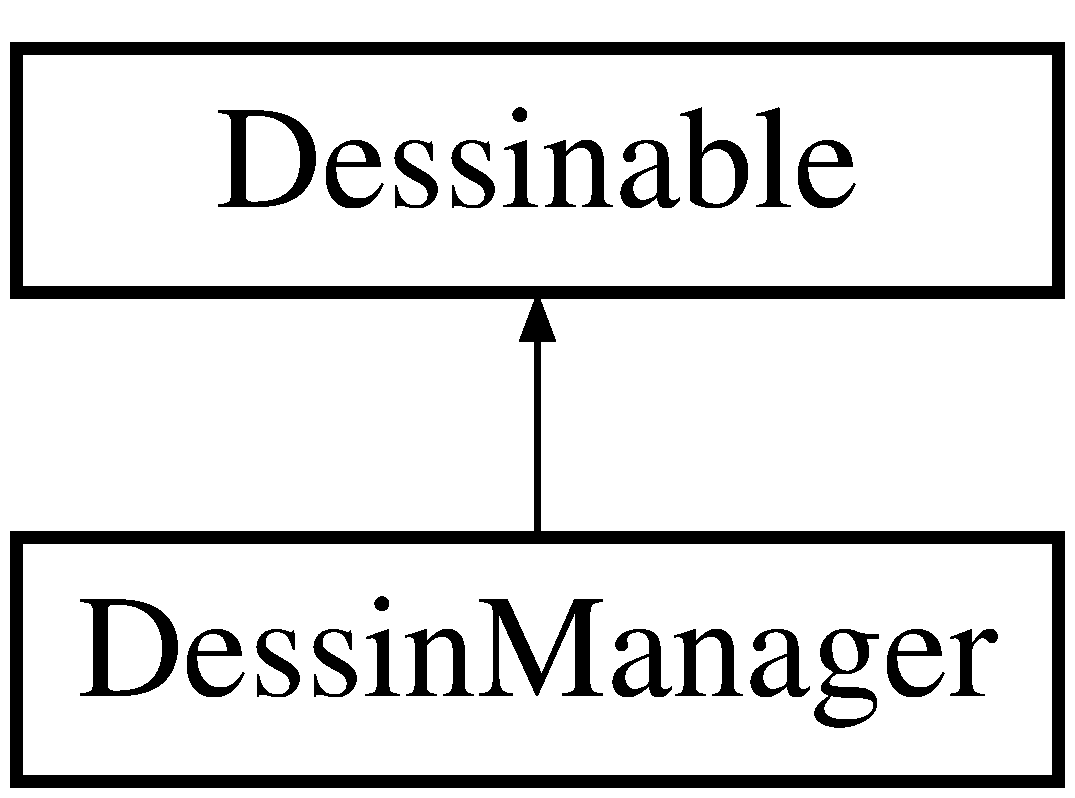
\includegraphics[height=2.000000cm]{class_dessin_manager}
\end{center}
\end{figure}
\subsection*{Fonctions membres publiques}
\begin{DoxyCompactItemize}
\item 
\hypertarget{class_dessin_manager_ac3fc2fa6c1ac46893076b6b4529b8511}{{\bfseries Dessin\+Manager} (\hyperlink{class_connexion}{Connexion} $\ast$c)}\label{class_dessin_manager_ac3fc2fa6c1ac46893076b6b4529b8511}

\item 
\hypertarget{class_dessin_manager_a14bbe90859f8171cdfaca8c7dd9120f7}{void {\bfseries dessiner\+Cercle} (const \hyperlink{class_cercle}{Cercle} \&c) const }\label{class_dessin_manager_a14bbe90859f8171cdfaca8c7dd9120f7}

\item 
\hypertarget{class_dessin_manager_a3b85589740f0972fdb6eb74967138c28}{void {\bfseries dessiner\+Triangle} (const \hyperlink{class_triangle}{Triangle} \&t) const }\label{class_dessin_manager_a3b85589740f0972fdb6eb74967138c28}

\item 
\hypertarget{class_dessin_manager_a84cad5d36cbafc15a8ec6d8ae73c85e7}{void {\bfseries dessiner\+Segment} (const \hyperlink{class_segment}{Segment} \&s) const }\label{class_dessin_manager_a84cad5d36cbafc15a8ec6d8ae73c85e7}

\item 
\hypertarget{class_dessin_manager_a47890198c16e30889abc5ce90fd24ad9}{void {\bfseries dessiner\+Polygone} (const \hyperlink{class_polygone}{Polygone} \&p) const }\label{class_dessin_manager_a47890198c16e30889abc5ce90fd24ad9}

\end{DoxyCompactItemize}


\subsection{Description détaillée}
The \hyperlink{class_dessin_manager}{Dessin\+Manager} class Cette classe est chargé de dessiner les formes géometriques. Le dessin est fait en envoyant les formes géometriques à un serveur distant afin que celui-\/ci dessine. 

La documentation de cette classe a été générée à partir des fichiers suivants \+:\begin{DoxyCompactItemize}
\item 
dessin\+Manager.\+h\item 
dessin\+Manager.\+cpp\end{DoxyCompactItemize}

\hypertarget{class_erreur}{\section{Référence de la classe Erreur}
\label{class_erreur}\index{Erreur@{Erreur}}
}
\subsection*{Fonctions membres publiques}
\begin{DoxyCompactItemize}
\item 
\hypertarget{class_erreur_a15bbbbc7e23e4ea5e6bdebe8e299e6be}{{\bfseries Erreur} (const char $\ast$message\+Erreur)}\label{class_erreur_a15bbbbc7e23e4ea5e6bdebe8e299e6be}

\item 
\hypertarget{class_erreur_a69e752f84bce4f8565f02c484cc4d55e}{{\bfseries operator string} () const }\label{class_erreur_a69e752f84bce4f8565f02c484cc4d55e}

\end{DoxyCompactItemize}
\subsection*{Attributs publics}
\begin{DoxyCompactItemize}
\item 
\hypertarget{class_erreur_a55ae1259e86044a99bb4e78109ece875}{char {\bfseries message} \mbox{[}1+L\+O\+N\+G\+U\+E\+U\+R\+M\+E\+S\+S\+A\+G\+E\mbox{]}}\label{class_erreur_a55ae1259e86044a99bb4e78109ece875}

\end{DoxyCompactItemize}
\subsection*{Attributs publics statiques}
\begin{DoxyCompactItemize}
\item 
\hypertarget{class_erreur_a4bad7e055ecc19aa6c7616ddf51d05dd}{static const int {\bfseries L\+O\+N\+G\+U\+E\+U\+R\+M\+E\+S\+S\+A\+G\+E} = 100}\label{class_erreur_a4bad7e055ecc19aa6c7616ddf51d05dd}

\end{DoxyCompactItemize}


La documentation de cette classe a été générée à partir des fichiers suivants \+:\begin{DoxyCompactItemize}
\item 
erreur.\+h\item 
erreur.\+cpp\end{DoxyCompactItemize}

\hypertarget{class_expert}{\section{Référence du modèle de la classe Expert$<$ retour, a\+Traiter $>$}
\label{class_expert}\index{Expert$<$ retour, a\+Traiter $>$@{Expert$<$ retour, a\+Traiter $>$}}
}
Graphe d'héritage de Expert$<$ retour, a\+Traiter $>$\+:\begin{figure}[H]
\begin{center}
\leavevmode
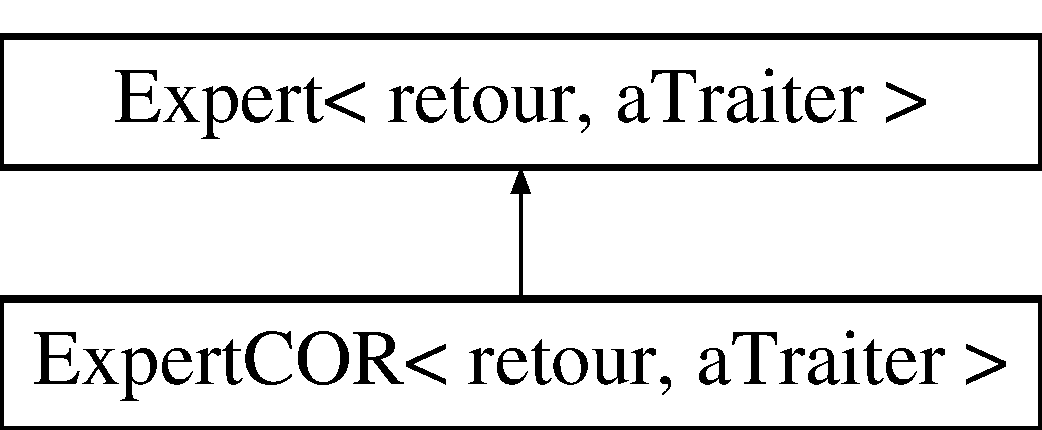
\includegraphics[height=2.000000cm]{class_expert}
\end{center}
\end{figure}
\subsection*{Fonctions membres publiques}
\begin{DoxyCompactItemize}
\item 
\hypertarget{class_expert_a87f345eef673e757f63bfa553c9525a1}{virtual retour $\ast$ {\bfseries traitement} (a\+Traiter \&objet) const =0}\label{class_expert_a87f345eef673e757f63bfa553c9525a1}

\end{DoxyCompactItemize}


La documentation de cette classe a été générée à partir du fichier suivant \+:\begin{DoxyCompactItemize}
\item 
chargement\+C\+O\+R/expert.\+h\end{DoxyCompactItemize}

\hypertarget{class_expert_chargement}{\section{Référence de la classe Expert\+Chargement}
\label{class_expert_chargement}\index{Expert\+Chargement@{Expert\+Chargement}}
}
Graphe d'héritage de Expert\+Chargement\+:\begin{figure}[H]
\begin{center}
\leavevmode
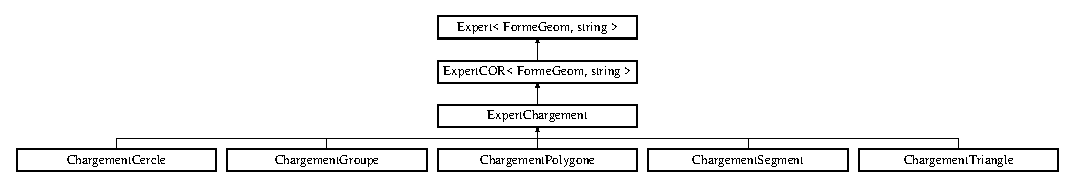
\includegraphics[height=2.083721cm]{class_expert_chargement}
\end{center}
\end{figure}
\subsection*{Fonctions membres publiques}
\begin{DoxyCompactItemize}
\item 
virtual \hyperlink{class_forme_geom}{Forme\+Geom} $\ast$ \hyperlink{class_expert_chargement_a7d7818bdd5f0a06b06bfc8047ec8fee5}{traitement\+Specialise} (string \&objet) const =0
\begin{DoxyCompactList}\small\item\em traitement1 \end{DoxyCompactList}\end{DoxyCompactItemize}


\subsection{Documentation des fonctions membres}
\hypertarget{class_expert_chargement_a7d7818bdd5f0a06b06bfc8047ec8fee5}{\index{Expert\+Chargement@{Expert\+Chargement}!traitement\+Specialise@{traitement\+Specialise}}
\index{traitement\+Specialise@{traitement\+Specialise}!Expert\+Chargement@{Expert\+Chargement}}
\subsubsection[{traitement\+Specialise}]{\setlength{\rightskip}{0pt plus 5cm}virtual {\bf Forme\+Geom}$\ast$ Expert\+Chargement\+::traitement\+Specialise (
\begin{DoxyParamCaption}
\item[{string \&}]{objet}
\end{DoxyParamCaption}
) const\hspace{0.3cm}{\ttfamily [pure virtual]}}}\label{class_expert_chargement_a7d7818bdd5f0a06b06bfc8047ec8fee5}


traitement1 


\begin{DoxyParams}{Paramètres}
{\em objet} & \\
\hline
\end{DoxyParams}
\begin{DoxyReturn}{Renvoie}
l'objet parsé ou N\+U\+L\+L si non trouvé. 
\end{DoxyReturn}


Implémente \hyperlink{class_expert_c_o_r_a7574fdd9c8321c8d7e4be820740d0760}{Expert\+C\+O\+R$<$ Forme\+Geom, string $>$}.



Implémenté dans \hyperlink{class_chargement_cercle_addd0be00b764eb7736aac2386bbafabd}{Chargement\+Cercle}, \hyperlink{class_chargement_groupe_aa0487a2d01a2c8022fbaf854e79bafd6}{Chargement\+Groupe}, \hyperlink{class_chargement_polygone_a66c85c1a8a6aba246a283aaa18bfddd4}{Chargement\+Polygone}, \hyperlink{class_chargement_triangle_a5a56b270c58404c940900c5d93237876}{Chargement\+Triangle}, et \hyperlink{class_chargement_segment_ab03da7e3e7870d2522d72095ae827135}{Chargement\+Segment}.



La documentation de cette classe a été générée à partir du fichier suivant \+:\begin{DoxyCompactItemize}
\item 
chargement\+C\+O\+R/expertchargement.\+h\end{DoxyCompactItemize}

\hypertarget{class_expert_c_o_r}{\section{Référence du modèle de la classe Expert\+C\+O\+R$<$ retour, a\+Traiter $>$}
\label{class_expert_c_o_r}\index{Expert\+C\+O\+R$<$ retour, a\+Traiter $>$@{Expert\+C\+O\+R$<$ retour, a\+Traiter $>$}}
}
Graphe d'héritage de Expert\+C\+O\+R$<$ retour, a\+Traiter $>$\+:\begin{figure}[H]
\begin{center}
\leavevmode
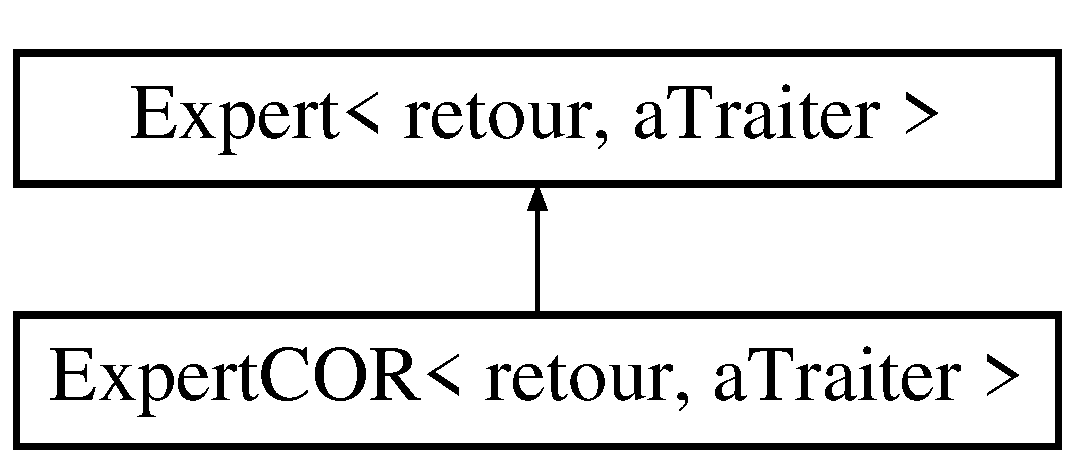
\includegraphics[height=2.000000cm]{class_expert_c_o_r}
\end{center}
\end{figure}
\subsection*{Fonctions membres publiques}
\begin{DoxyCompactItemize}
\item 
\hypertarget{class_expert_c_o_r_aac1c145afdd4e0ae81fd484c05ea9e64}{void {\bfseries ajouter\+Suivant} (\hyperlink{class_expert_c_o_r}{Expert\+C\+O\+R}$<$ retour, a\+Traiter $>$ $\ast$suiv)}\label{class_expert_c_o_r_aac1c145afdd4e0ae81fd484c05ea9e64}

\item 
\hypertarget{class_expert_c_o_r_aca5940c9d0b1fe6ce0f2318636a19ac5}{virtual retour $\ast$ {\bfseries traitement} (a\+Traiter \&objet) const }\label{class_expert_c_o_r_aca5940c9d0b1fe6ce0f2318636a19ac5}

\item 
virtual retour $\ast$ \hyperlink{class_expert_c_o_r_a7574fdd9c8321c8d7e4be820740d0760}{traitement\+Specialise} (a\+Traiter \&objet) const =0
\begin{DoxyCompactList}\small\item\em traitement1 Si pas de suivant et echec du traitement, lève l'exception traitement impossible \end{DoxyCompactList}\end{DoxyCompactItemize}


\subsection{Documentation des fonctions membres}
\hypertarget{class_expert_c_o_r_a7574fdd9c8321c8d7e4be820740d0760}{\index{Expert\+C\+O\+R@{Expert\+C\+O\+R}!traitement\+Specialise@{traitement\+Specialise}}
\index{traitement\+Specialise@{traitement\+Specialise}!Expert\+C\+O\+R@{Expert\+C\+O\+R}}
\subsubsection[{traitement\+Specialise}]{\setlength{\rightskip}{0pt plus 5cm}template$<$class retour, class a\+Traiter$>$ virtual retour$\ast$ {\bf Expert\+C\+O\+R}$<$ retour, a\+Traiter $>$\+::traitement\+Specialise (
\begin{DoxyParamCaption}
\item[{a\+Traiter \&}]{objet}
\end{DoxyParamCaption}
) const\hspace{0.3cm}{\ttfamily [pure virtual]}}}\label{class_expert_c_o_r_a7574fdd9c8321c8d7e4be820740d0760}


traitement1 Si pas de suivant et echec du traitement, lève l'exception traitement impossible 


\begin{DoxyParams}{Paramètres}
{\em objet} & \\
\hline
\end{DoxyParams}
\begin{DoxyReturn}{Renvoie}

\end{DoxyReturn}


Implémenté dans \hyperlink{class_expert_chargement_a7d7818bdd5f0a06b06bfc8047ec8fee5}{Expert\+Chargement}, \hyperlink{class_chargement_cercle_addd0be00b764eb7736aac2386bbafabd}{Chargement\+Cercle}, \hyperlink{class_chargement_groupe_aa0487a2d01a2c8022fbaf854e79bafd6}{Chargement\+Groupe}, \hyperlink{class_chargement_polygone_a66c85c1a8a6aba246a283aaa18bfddd4}{Chargement\+Polygone}, \hyperlink{class_chargement_triangle_a5a56b270c58404c940900c5d93237876}{Chargement\+Triangle}, et \hyperlink{class_chargement_segment_ab03da7e3e7870d2522d72095ae827135}{Chargement\+Segment}.



La documentation de cette classe a été générée à partir du fichier suivant \+:\begin{DoxyCompactItemize}
\item 
chargement\+C\+O\+R/expertcor.\+h\end{DoxyCompactItemize}

\hypertarget{class_facade}{\section{Référence du modèle de la classe Facade$<$ retour, a\+Traiter $>$}
\label{class_facade}\index{Facade$<$ retour, a\+Traiter $>$@{Facade$<$ retour, a\+Traiter $>$}}
}
\subsection*{Fonctions membres publiques}
\begin{DoxyCompactItemize}
\item 
\hypertarget{class_facade_a2765bcffe76eefe10056046fa0e1310d}{retour $\ast$ {\bfseries run} ()}\label{class_facade_a2765bcffe76eefe10056046fa0e1310d}

\end{DoxyCompactItemize}
\subsection*{Attributs protégés}
\begin{DoxyCompactItemize}
\item 
\hypertarget{class_facade_a44429d44d23a014898a344f1d8ee5ea3}{\hyperlink{class_expert_c_o_r}{Expert\+C\+O\+R}$<$ retour, a\+Traiter $>$ $\ast$ {\bfseries \+\_\+first}}\label{class_facade_a44429d44d23a014898a344f1d8ee5ea3}

\item 
\hypertarget{class_facade_af1abc64b47fc587b2b2a0db76c7c8ac9}{a\+Traiter {\bfseries \+\_\+objet}}\label{class_facade_af1abc64b47fc587b2b2a0db76c7c8ac9}

\end{DoxyCompactItemize}


La documentation de cette classe a été générée à partir du fichier suivant \+:\begin{DoxyCompactItemize}
\item 
chargement\+C\+O\+R/facade.\+h\end{DoxyCompactItemize}

\hypertarget{class_forme_composee}{\section{Référence du modèle de la classe Forme\+Composee$<$ C, T $>$}
\label{class_forme_composee}\index{Forme\+Composee$<$ C, T $>$@{Forme\+Composee$<$ C, T $>$}}
}
Graphe d'héritage de Forme\+Composee$<$ C, T $>$\+:\begin{figure}[H]
\begin{center}
\leavevmode
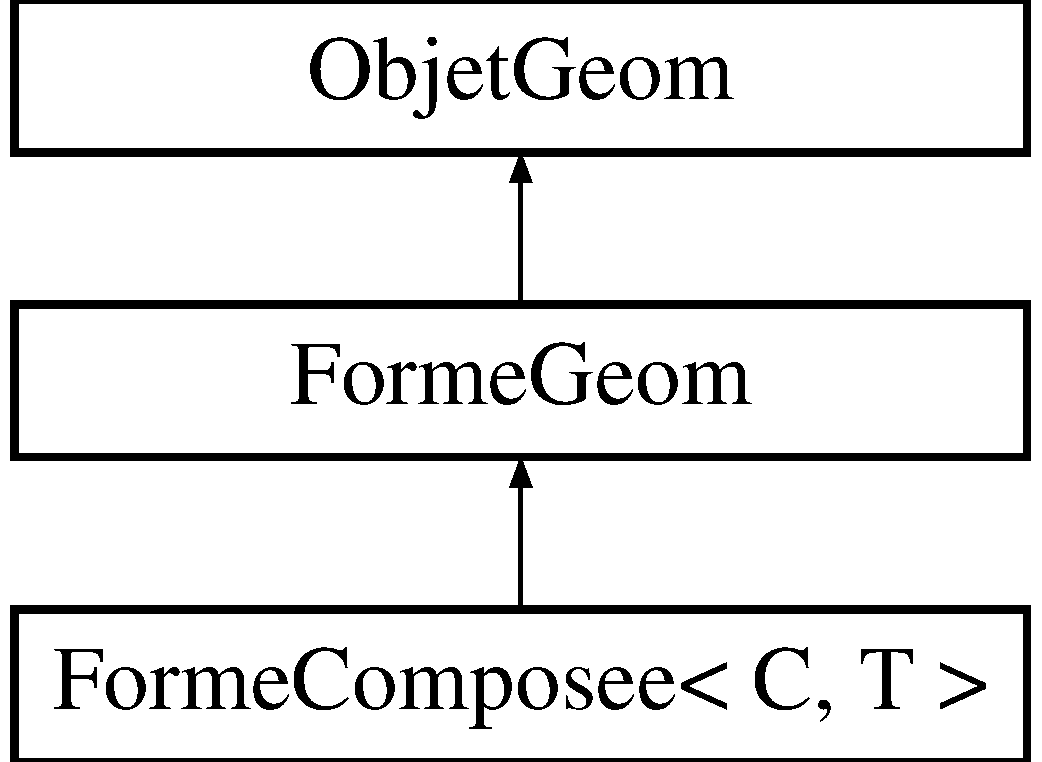
\includegraphics[height=3.000000cm]{class_forme_composee}
\end{center}
\end{figure}
\subsection*{Fonctions membres publiques}
\begin{DoxyCompactItemize}
\item 
\hypertarget{class_forme_composee_ac2e1bc2fe2bd15ea64f54437506efc23}{{\bfseries Forme\+Composee} (const Couleurs\+::\+Couleur \&couleur)}\label{class_forme_composee_ac2e1bc2fe2bd15ea64f54437506efc23}

\item 
\hypertarget{class_forme_composee_a1cf7d4f5a75aca415db4c82b4ce58bc2}{{\bfseries Forme\+Composee} (const Couleurs\+::\+Couleur \&couleur, const vector$<$ C $\ast$ $>$ \&comp)}\label{class_forme_composee_a1cf7d4f5a75aca415db4c82b4ce58bc2}

\item 
\hypertarget{class_forme_composee_a2b08c0c0862c3add1a8acd73d0636d4e}{int {\bfseries get\+Nb\+Elem} () const }\label{class_forme_composee_a2b08c0c0862c3add1a8acd73d0636d4e}

\item 
\hypertarget{class_forme_composee_ac2eca4ffa3fa09c1b1c3b87b5536cf93}{vector$<$ C $\ast$ $>$ {\bfseries get\+Composants} () const }\label{class_forme_composee_ac2eca4ffa3fa09c1b1c3b87b5536cf93}

\item 
\hypertarget{class_forme_composee_a77ec5853c218184f5cd4fd44b98c99a1}{virtual \hyperlink{class_forme_composee}{Forme\+Composee}$<$ C, T $>$ $\ast$ {\bfseries rotation} (const \hyperlink{class_point}{Point} \&p, const \hyperlink{class_angle}{Angle} \&angle) const }\label{class_forme_composee_a77ec5853c218184f5cd4fd44b98c99a1}

\item 
\hypertarget{class_forme_composee_ac9092340280d7c1dc41aef2468a30752}{virtual \hyperlink{class_forme_composee}{Forme\+Composee}$<$ C, T $>$ $\ast$ {\bfseries homothetie} (const \hyperlink{class_point}{Point} \&p, const double \&d) const }\label{class_forme_composee_ac9092340280d7c1dc41aef2468a30752}

\item 
\hypertarget{class_forme_composee_a7657bdc10df7702ac89646347c273438}{virtual \hyperlink{class_forme_composee}{Forme\+Composee}$<$ C, T $>$ $\ast$ {\bfseries translation} (const \hyperlink{class_vecteur}{Vecteur} \&v) const }\label{class_forme_composee_a7657bdc10df7702ac89646347c273438}

\end{DoxyCompactItemize}
\subsection*{Attributs protégés}
\begin{DoxyCompactItemize}
\item 
\hypertarget{class_forme_composee_a5d6afdf045e0fcec2071520004aacc40}{vector$<$ C $\ast$ $>$ {\bfseries \+\_\+composants}}\label{class_forme_composee_a5d6afdf045e0fcec2071520004aacc40}

\end{DoxyCompactItemize}
\subsection*{Membres hérités additionnels}


La documentation de cette classe a été générée à partir du fichier suivant \+:\begin{DoxyCompactItemize}
\item 
formecomposee.\+h\end{DoxyCompactItemize}

\hypertarget{class_forme_geom}{\section{Référence de la classe Forme\+Geom}
\label{class_forme_geom}\index{Forme\+Geom@{Forme\+Geom}}
}
Graphe d'héritage de Forme\+Geom\+:\begin{figure}[H]
\begin{center}
\leavevmode
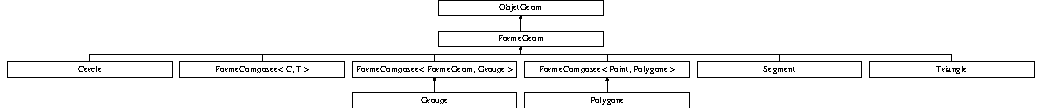
\includegraphics[height=1.447028cm]{class_forme_geom}
\end{center}
\end{figure}
\subsection*{Fonctions membres publiques}
\begin{DoxyCompactItemize}
\item 
\hypertarget{class_forme_geom_a522c46b60f03b3abaeb6d331d39b7980}{{\bfseries Forme\+Geom} (const Couleurs\+::\+Couleur \&coul)}\label{class_forme_geom_a522c46b60f03b3abaeb6d331d39b7980}

\item 
\hypertarget{class_forme_geom_a5f088772aeb5d24bf79b19f13239d47d}{\hyperlink{class_groupe}{Groupe} $\ast$ {\bfseries appartient\+A} () const }\label{class_forme_geom_a5f088772aeb5d24bf79b19f13239d47d}

\item 
\hypertarget{class_forme_geom_a3365e177e6dd0b1096669b425b28f47e}{void {\bfseries set\+Appartient\+A} (\hyperlink{class_groupe}{Groupe} $\ast$g)}\label{class_forme_geom_a3365e177e6dd0b1096669b425b28f47e}

\item 
\hypertarget{class_forme_geom_ad53f396ba18b26873e272856ecf72f23}{void {\bfseries set\+Couleur} (const Couleurs\+::\+Couleur \&c)}\label{class_forme_geom_ad53f396ba18b26873e272856ecf72f23}

\item 
\hypertarget{class_forme_geom_a256b60ef99c5febe866084ce4b928f3e}{Couleurs\+::\+Couleur {\bfseries get\+Couleur} () const }\label{class_forme_geom_a256b60ef99c5febe866084ce4b928f3e}

\item 
\hypertarget{class_forme_geom_a14e52f725e4eaf66d970aa67bae35812}{virtual \hyperlink{class_forme_geom}{Forme\+Geom} $\ast$ {\bfseries rotation} (const \hyperlink{class_point}{Point} \&p, const \hyperlink{class_angle}{Angle} \&angle) const =0}\label{class_forme_geom_a14e52f725e4eaf66d970aa67bae35812}

\item 
\hypertarget{class_forme_geom_abb0e0d909fc7916fdd31747780ebf44d}{virtual \hyperlink{class_forme_geom}{Forme\+Geom} $\ast$ {\bfseries homothetie} (const \hyperlink{class_point}{Point} \&p, const double \&scale) const =0}\label{class_forme_geom_abb0e0d909fc7916fdd31747780ebf44d}

\item 
\hypertarget{class_forme_geom_adebc8e4fe8dab62f4a4b03d7d3ec7230}{virtual \hyperlink{class_forme_geom}{Forme\+Geom} $\ast$ {\bfseries translation} (const \hyperlink{class_vecteur}{Vecteur} \&v) const =0}\label{class_forme_geom_adebc8e4fe8dab62f4a4b03d7d3ec7230}

\item 
\hypertarget{class_forme_geom_acca1a53eaf6886236a61541fed4b36f1}{virtual \hyperlink{class_forme_geom}{Forme\+Geom} $\ast$ {\bfseries clone} () const =0}\label{class_forme_geom_acca1a53eaf6886236a61541fed4b36f1}

\item 
\hypertarget{class_forme_geom_a1812fc8597994c1bc75a577785c356dd}{virtual double {\bfseries aire} () const =0}\label{class_forme_geom_a1812fc8597994c1bc75a577785c356dd}

\item 
\hypertarget{class_forme_geom_a80fabca42026f9a5d72fd12988da164e}{virtual void {\bfseries dessin} (const \hyperlink{class_dessinable}{Dessinable} \&) const =0}\label{class_forme_geom_a80fabca42026f9a5d72fd12988da164e}

\item 
\hypertarget{class_forme_geom_a25ff69dc148f04e4d9bc5e5305a08d10}{void {\bfseries sauvegarder} (const string nom\+De\+Fichier) const }\label{class_forme_geom_a25ff69dc148f04e4d9bc5e5305a08d10}

\end{DoxyCompactItemize}
\subsection*{Fonctions membres publiques statiques}
\begin{DoxyCompactItemize}
\item 
\hypertarget{class_forme_geom_a874df9fef2c3f6dd1b4eaf1496f6870b}{static \hyperlink{class_forme_geom}{Forme\+Geom} $\ast$ {\bfseries chargement} (const string \&nom\+De\+Fichier)}\label{class_forme_geom_a874df9fef2c3f6dd1b4eaf1496f6870b}

\end{DoxyCompactItemize}
\subsection*{Attributs protégés}
\begin{DoxyCompactItemize}
\item 
\hypertarget{class_forme_geom_a81f31ae59515184c36eee84bf2191472}{Couleurs\+::\+Couleur {\bfseries \+\_\+couleur}}\label{class_forme_geom_a81f31ae59515184c36eee84bf2191472}

\item 
\hypertarget{class_forme_geom_a4f7af3f9b22145883ea319eee243dfd4}{\hyperlink{class_groupe}{Groupe} $\ast$ {\bfseries \+\_\+appartient\+A}}\label{class_forme_geom_a4f7af3f9b22145883ea319eee243dfd4}

\end{DoxyCompactItemize}


La documentation de cette classe a été générée à partir des fichiers suivants \+:\begin{DoxyCompactItemize}
\item 
formegeom.\+h\item 
formegeom.\+cpp\end{DoxyCompactItemize}

\hypertarget{class_groupe}{\section{Référence de la classe Groupe}
\label{class_groupe}\index{Groupe@{Groupe}}
}


The \hyperlink{class_groupe}{Groupe} class Un groupe est un ensemble de formes composées. Chaque forme le constituant est une copie de la forme originale. L'ajout d'une forme dans un groupe change sa couleur pour celle du groupe.  




{\ttfamily \#include $<$groupe.\+h$>$}

Graphe d'héritage de Groupe\+:\begin{figure}[H]
\begin{center}
\leavevmode
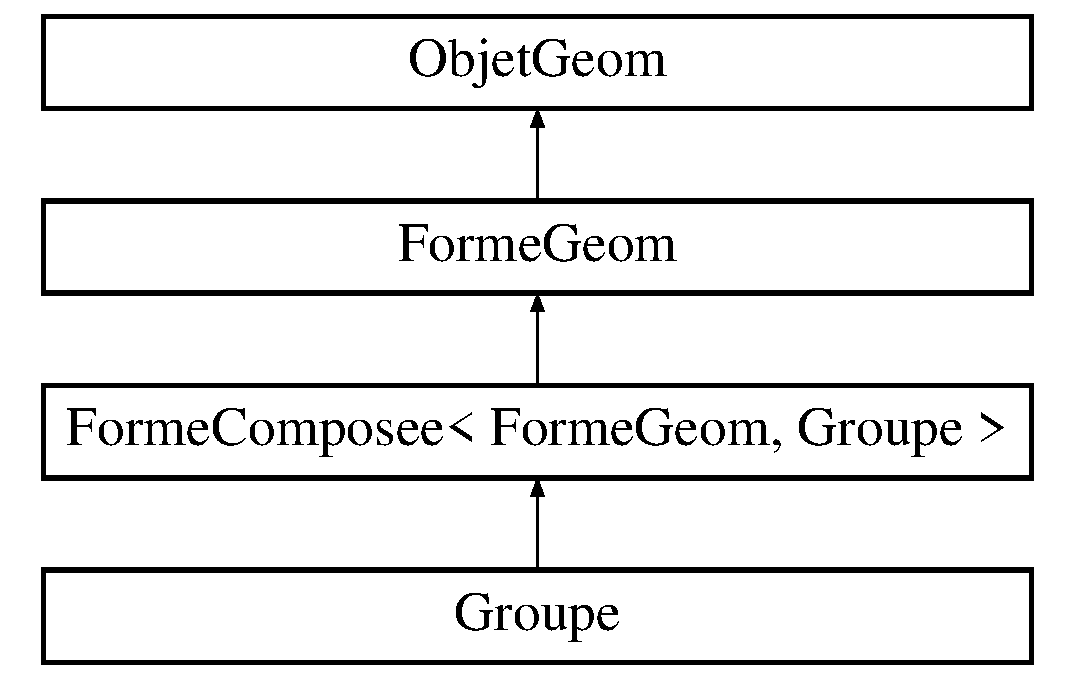
\includegraphics[height=4.000000cm]{class_groupe}
\end{center}
\end{figure}
\subsection*{Fonctions membres publiques}
\begin{DoxyCompactItemize}
\item 
\hypertarget{class_groupe_aa7f2a1ce7018f40ee6c518f62aa5b8d3}{{\bfseries Groupe} (const \hyperlink{class_forme_composee}{Forme\+Composee}$<$ \hyperlink{class_forme_geom}{Forme\+Geom}, \hyperlink{class_groupe}{Groupe} $>$ \&f)}\label{class_groupe_aa7f2a1ce7018f40ee6c518f62aa5b8d3}

\item 
\hypertarget{class_groupe_adf726dba5919371e203f34441215ef2d}{{\bfseries Groupe} (const \hyperlink{class_groupe}{Groupe} \&)}\label{class_groupe_adf726dba5919371e203f34441215ef2d}

\item 
\hypertarget{class_groupe_a659615b48f68f6f0ff8052ae4201ac67}{{\bfseries Groupe} (const Couleurs\+::\+Couleur \&coul)}\label{class_groupe_a659615b48f68f6f0ff8052ae4201ac67}

\item 
\hypertarget{class_groupe_a923d63c16045730cc5276a5be8e04685}{virtual void {\bfseries ajouter} (const \hyperlink{class_forme_geom}{Forme\+Geom} \&f)}\label{class_groupe_a923d63c16045730cc5276a5be8e04685}

\item 
void \hyperlink{class_groupe_a8a31cdfca2e4729ecaceebb3038ba931}{supprimer} (const double \&index)
\begin{DoxyCompactList}\small\item\em \hyperlink{class_groupe_a8a31cdfca2e4729ecaceebb3038ba931}{Groupe\+::supprimer} enl�ve la forme de la liste et de la m�moire. \end{DoxyCompactList}\item 
void \hyperlink{class_groupe_a0ea16776237c99ea14eb910c5d053e88}{enlever} (const \hyperlink{class_forme_geom}{Forme\+Geom} $\ast$forme)
\begin{DoxyCompactList}\small\item\em \hyperlink{class_groupe_a0ea16776237c99ea14eb910c5d053e88}{Groupe\+::enlever} enl�ve forme du groupe, ne le supprime pas de la m�moire. \end{DoxyCompactList}\item 
\hyperlink{class_forme_geom}{Forme\+Geom} $\ast$ \hyperlink{class_groupe_ace75101b0417cead91c911682537c62f}{get} (size\+\_\+t i) const 
\begin{DoxyCompactList}\small\item\em get \end{DoxyCompactList}\item 
\hypertarget{class_groupe_ae81ebd4b7292c02e909aec794f676643}{virtual string {\bfseries to\+String} () const }\label{class_groupe_ae81ebd4b7292c02e909aec794f676643}

\item 
\hypertarget{class_groupe_ab5184897ea2f56b4f280852e4665f824}{virtual void {\bfseries dessin} (const \hyperlink{class_dessinable}{Dessinable} \&d) const }\label{class_groupe_ab5184897ea2f56b4f280852e4665f824}

\item 
\hypertarget{class_groupe_aa9a817d398da48c63dd8c5435be0edfa}{virtual double {\bfseries aire} () const }\label{class_groupe_aa9a817d398da48c63dd8c5435be0edfa}

\item 
\hypertarget{class_groupe_a2ee3c8904c199b3bdc777817286f1c44}{virtual \hyperlink{class_groupe}{Groupe} $\ast$ {\bfseries clone} () const }\label{class_groupe_a2ee3c8904c199b3bdc777817286f1c44}

\item 
\hypertarget{class_groupe_a99dd414922635dcc0585aabb2a330f63}{virtual \hyperlink{class_groupe_a99dd414922635dcc0585aabb2a330f63}{$\sim$\+Groupe} ()}\label{class_groupe_a99dd414922635dcc0585aabb2a330f63}

\begin{DoxyCompactList}\small\item\em \hyperlink{class_groupe_a99dd414922635dcc0585aabb2a330f63}{Groupe\+::$\sim$\+Groupe} Rien � faire car les objets dans le groupe doivent �tre g�r�s en dehors de celui-\/ci. \end{DoxyCompactList}\end{DoxyCompactItemize}
\subsection*{Membres hérités additionnels}


\subsection{Description détaillée}
The \hyperlink{class_groupe}{Groupe} class Un groupe est un ensemble de formes composées. Chaque forme le constituant est une copie de la forme originale. L'ajout d'une forme dans un groupe change sa couleur pour celle du groupe. 

\subsection{Documentation des fonctions membres}
\hypertarget{class_groupe_a0ea16776237c99ea14eb910c5d053e88}{\index{Groupe@{Groupe}!enlever@{enlever}}
\index{enlever@{enlever}!Groupe@{Groupe}}
\subsubsection[{enlever}]{\setlength{\rightskip}{0pt plus 5cm}void Groupe\+::enlever (
\begin{DoxyParamCaption}
\item[{const {\bf Forme\+Geom} $\ast$}]{forme}
\end{DoxyParamCaption}
)}}\label{class_groupe_a0ea16776237c99ea14eb910c5d053e88}


\hyperlink{class_groupe_a0ea16776237c99ea14eb910c5d053e88}{Groupe\+::enlever} enl�ve forme du groupe, ne le supprime pas de la m�moire. 


\begin{DoxyParams}{Paramètres}
{\em forme} & \\
\hline
\end{DoxyParams}
\hypertarget{class_groupe_ace75101b0417cead91c911682537c62f}{\index{Groupe@{Groupe}!get@{get}}
\index{get@{get}!Groupe@{Groupe}}
\subsubsection[{get}]{\setlength{\rightskip}{0pt plus 5cm}{\bf Forme\+Geom} $\ast$ Groupe\+::get (
\begin{DoxyParamCaption}
\item[{size\+\_\+t}]{i}
\end{DoxyParamCaption}
) const\hspace{0.3cm}{\ttfamily [inline]}}}\label{class_groupe_ace75101b0417cead91c911682537c62f}


get 


\begin{DoxyParams}{Paramètres}
{\em i} & \\
\hline
\end{DoxyParams}
\begin{DoxyReturn}{Renvoie}
l'objet à la position i, N\+U\+L\+L si la position est mauvaise. Attention ne pas détruire l'objet avant que le groupe ne soit lui même détruit. 
\end{DoxyReturn}
\hypertarget{class_groupe_a8a31cdfca2e4729ecaceebb3038ba931}{\index{Groupe@{Groupe}!supprimer@{supprimer}}
\index{supprimer@{supprimer}!Groupe@{Groupe}}
\subsubsection[{supprimer}]{\setlength{\rightskip}{0pt plus 5cm}void Groupe\+::supprimer (
\begin{DoxyParamCaption}
\item[{const double \&}]{index}
\end{DoxyParamCaption}
)}}\label{class_groupe_a8a31cdfca2e4729ecaceebb3038ba931}


\hyperlink{class_groupe_a8a31cdfca2e4729ecaceebb3038ba931}{Groupe\+::supprimer} enl�ve la forme de la liste et de la m�moire. 


\begin{DoxyParams}{Paramètres}
{\em f} & \\
\hline
\end{DoxyParams}


La documentation de cette classe a été générée à partir des fichiers suivants \+:\begin{DoxyCompactItemize}
\item 
groupe.\+h\item 
groupe.\+cpp\end{DoxyCompactItemize}

\hypertarget{class_main_window}{\section{Référence de la classe Main\+Window}
\label{class_main_window}\index{Main\+Window@{Main\+Window}}
}
Graphe d'héritage de Main\+Window\+:\begin{figure}[H]
\begin{center}
\leavevmode
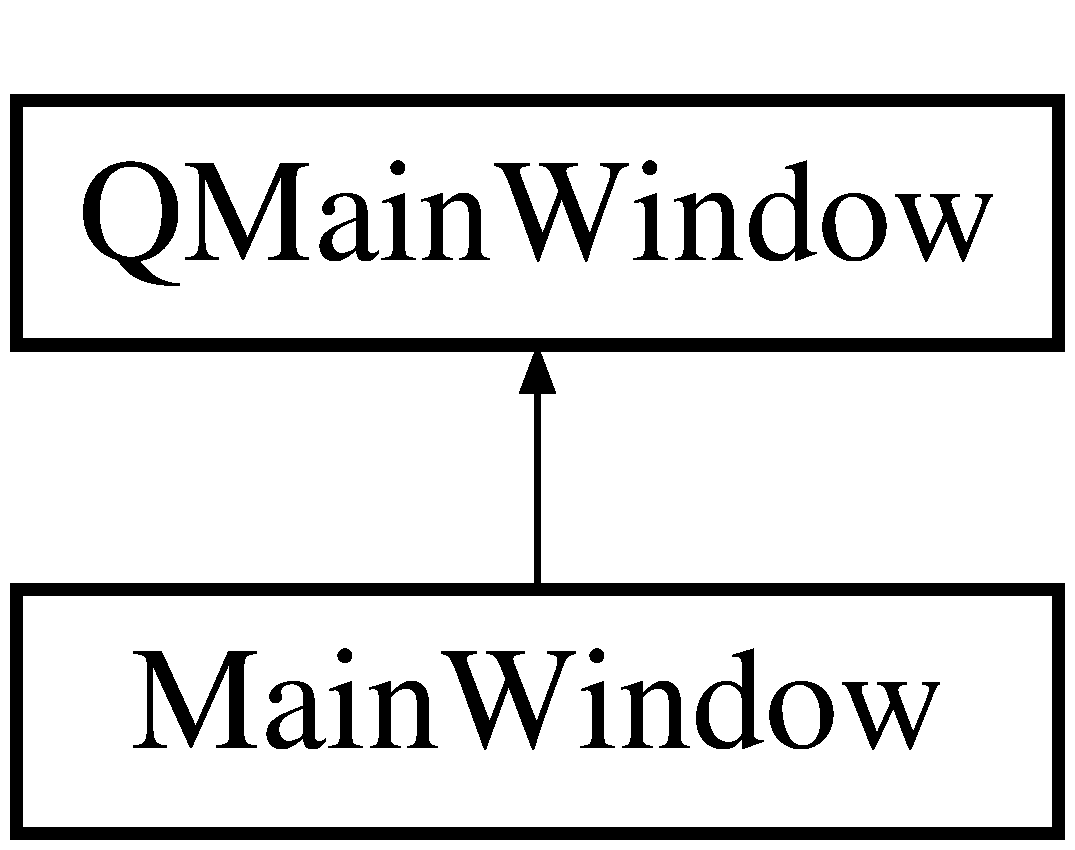
\includegraphics[height=2.000000cm]{class_main_window}
\end{center}
\end{figure}
\subsection*{Fonctions membres publiques}
\begin{DoxyCompactItemize}
\item 
\hypertarget{class_main_window_a8b244be8b7b7db1b08de2a2acb9409db}{{\bfseries Main\+Window} (Q\+Widget $\ast$parent=0)}\label{class_main_window_a8b244be8b7b7db1b08de2a2acb9409db}

\end{DoxyCompactItemize}


La documentation de cette classe a été générée à partir des fichiers suivants \+:\begin{DoxyCompactItemize}
\item 
mainwindow.\+h\item 
mainwindow.\+cpp\end{DoxyCompactItemize}

\hypertarget{class_matrice_carree2}{\section{Référence de la classe Matrice\+Carree2}
\label{class_matrice_carree2}\index{Matrice\+Carree2@{Matrice\+Carree2}}
}
\subsection*{Fonctions membres publiques}
\begin{DoxyCompactItemize}
\item 
\hypertarget{class_matrice_carree2_a9d9bf4f1ef2cef83ced50ca797f765c2}{{\bfseries Matrice\+Carree2} (const \hyperlink{class_vecteur}{Vecteur} \&v1, const \hyperlink{class_vecteur}{Vecteur} \&v2)}\label{class_matrice_carree2_a9d9bf4f1ef2cef83ced50ca797f765c2}

\item 
\hypertarget{class_matrice_carree2_a1a28b1973d81290e9ac9cad3c17d2699}{{\bfseries Matrice\+Carree2} (const double \&x1, const double \&y1, const double \&x2, const double \&y2)}\label{class_matrice_carree2_a1a28b1973d81290e9ac9cad3c17d2699}

\item 
\hypertarget{class_matrice_carree2_a466c402680f683fa16b64723ec5a7e17}{\hyperlink{class_vecteur}{Vecteur} {\bfseries get\+L1} () const }\label{class_matrice_carree2_a466c402680f683fa16b64723ec5a7e17}

\item 
\hypertarget{class_matrice_carree2_aa7e0d89fbb3608ec81df059fb771c944}{\hyperlink{class_vecteur}{Vecteur} {\bfseries get\+L2} () const }\label{class_matrice_carree2_aa7e0d89fbb3608ec81df059fb771c944}

\item 
\hypertarget{class_matrice_carree2_aeda80c8a5ed6c8b0c20916e18ce00897}{const \hyperlink{class_vecteur}{Vecteur} {\bfseries operator$\ast$} (const \hyperlink{class_vecteur}{Vecteur} \&v)}\label{class_matrice_carree2_aeda80c8a5ed6c8b0c20916e18ce00897}

\end{DoxyCompactItemize}
\subsection*{Fonctions membres publiques statiques}
\begin{DoxyCompactItemize}
\item 
\hypertarget{class_matrice_carree2_aa58d3933eb2fa12915ea3a048d6b28d0}{static \hyperlink{class_matrice_carree2}{Matrice\+Carree2} {\bfseries get\+Matrice\+Rotation} (const \hyperlink{class_angle}{Angle} \&a)}\label{class_matrice_carree2_aa58d3933eb2fa12915ea3a048d6b28d0}

\end{DoxyCompactItemize}
\subsection*{Attributs publics statiques}
\begin{DoxyCompactItemize}
\item 
\hypertarget{class_matrice_carree2_aa733d1b47f9284bb4cafe32ca6a3cc2a}{static const \hyperlink{class_matrice_carree2}{Matrice\+Carree2} {\bfseries matrice\+Identitee}}\label{class_matrice_carree2_aa733d1b47f9284bb4cafe32ca6a3cc2a}

\end{DoxyCompactItemize}


La documentation de cette classe a été générée à partir des fichiers suivants \+:\begin{DoxyCompactItemize}
\item 
matricecarree2.\+h\item 
matricecarree2.\+cpp\end{DoxyCompactItemize}

\hypertarget{class_objet_geom}{\section{Référence de la classe Objet\+Geom}
\label{class_objet_geom}\index{Objet\+Geom@{Objet\+Geom}}
}
Graphe d'héritage de Objet\+Geom\+:\begin{figure}[H]
\begin{center}
\leavevmode
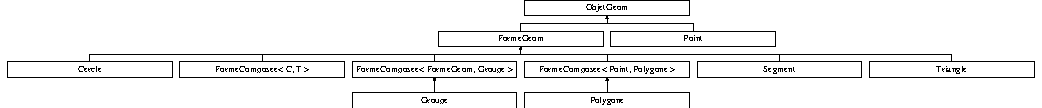
\includegraphics[height=1.447028cm]{class_objet_geom}
\end{center}
\end{figure}
\subsection*{Fonctions membres publiques}
\begin{DoxyCompactItemize}
\item 
\hypertarget{class_objet_geom_afee16245fc1bdf9ecd84e3b9eee28eda}{virtual \hyperlink{class_objet_geom}{Objet\+Geom} $\ast$ {\bfseries rotation} (const \hyperlink{class_point}{Point} \&p, const \hyperlink{class_angle}{Angle} \&angle) const =0}\label{class_objet_geom_afee16245fc1bdf9ecd84e3b9eee28eda}

\item 
\hypertarget{class_objet_geom_a5226444eaac635d6eda0b4b3738ca9f4}{virtual \hyperlink{class_objet_geom}{Objet\+Geom} $\ast$ {\bfseries homothetie} (const \hyperlink{class_point}{Point} \&p, const double \&scale) const =0}\label{class_objet_geom_a5226444eaac635d6eda0b4b3738ca9f4}

\item 
\hypertarget{class_objet_geom_a42e5bc7bc7c1b187daa45f4fc397ae99}{virtual \hyperlink{class_objet_geom}{Objet\+Geom} $\ast$ {\bfseries translation} (const \hyperlink{class_vecteur}{Vecteur} \&v) const =0}\label{class_objet_geom_a42e5bc7bc7c1b187daa45f4fc397ae99}

\item 
\hypertarget{class_objet_geom_ab70623d99c3a6646f5b6f8a94adf1246}{virtual std\+::string {\bfseries to\+String} () const =0}\label{class_objet_geom_ab70623d99c3a6646f5b6f8a94adf1246}

\item 
\hypertarget{class_objet_geom_ae86398cfaa3852ec5f604102d3a2684c}{virtual \hyperlink{class_objet_geom}{Objet\+Geom} $\ast$ {\bfseries clone} () const =0}\label{class_objet_geom_ae86398cfaa3852ec5f604102d3a2684c}

\end{DoxyCompactItemize}


La documentation de cette classe a été générée à partir du fichier suivant \+:\begin{DoxyCompactItemize}
\item 
objetgeom.\+h\end{DoxyCompactItemize}

\hypertarget{class_point}{\section{Référence de la classe Point}
\label{class_point}\index{Point@{Point}}
}
Graphe d'héritage de Point\+:\begin{figure}[H]
\begin{center}
\leavevmode
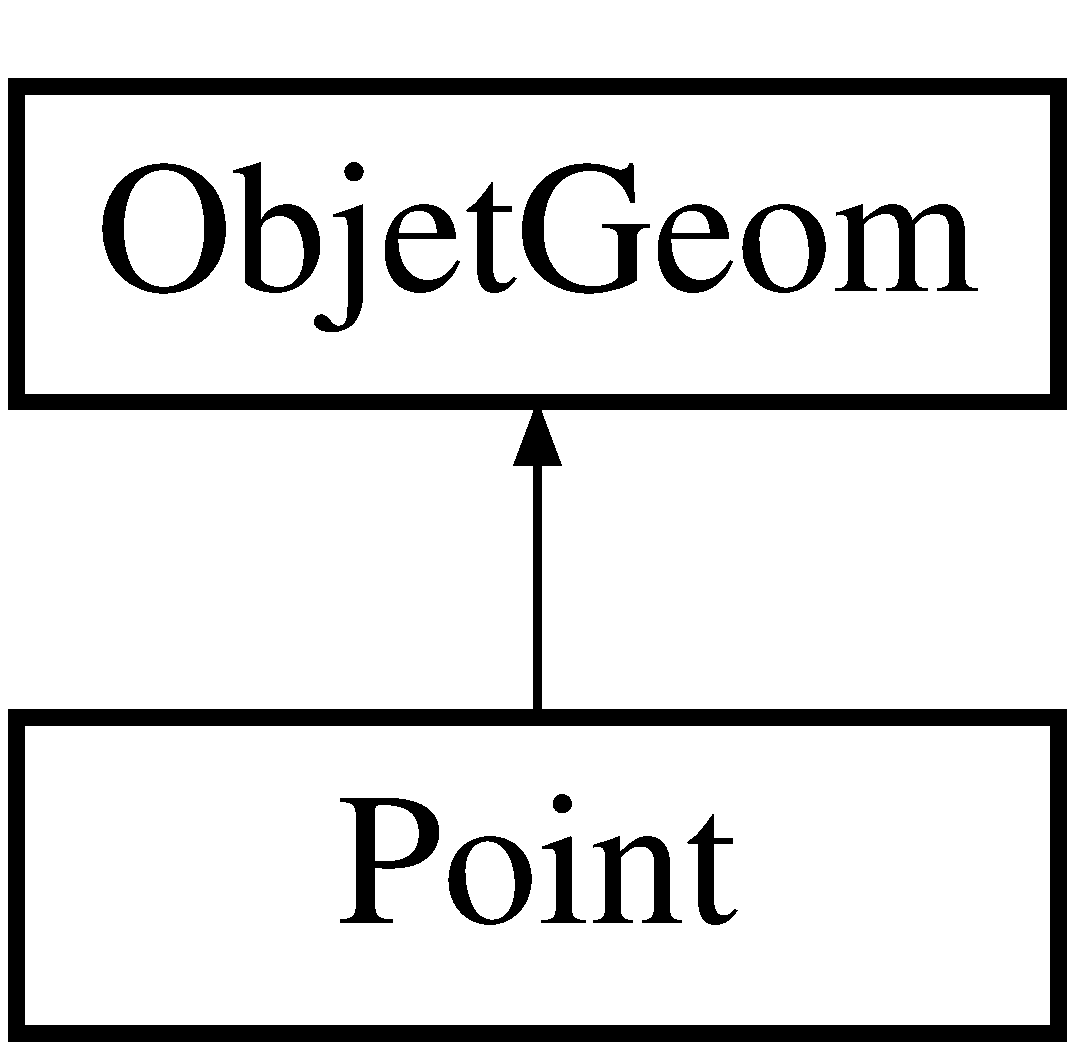
\includegraphics[height=2.000000cm]{class_point}
\end{center}
\end{figure}
\subsection*{Fonctions membres publiques}
\begin{DoxyCompactItemize}
\item 
\hypertarget{class_point_af0c0f20db1616447bc78184ed537ef6e}{{\bfseries Point} (const \hyperlink{class_point}{Point} \&p)}\label{class_point_af0c0f20db1616447bc78184ed537ef6e}

\item 
\hypertarget{class_point_a6761ef774ae06ee3226c8050756e0e03}{{\bfseries Point} (const \hyperlink{class_vecteur}{Vecteur} \&)}\label{class_point_a6761ef774ae06ee3226c8050756e0e03}

\item 
\hypertarget{class_point_a78b55e8d5466bb8c2cf60fa55f2562ff}{{\bfseries Point} (double x, double y)}\label{class_point_a78b55e8d5466bb8c2cf60fa55f2562ff}

\item 
\hypertarget{class_point_a4663f6c2c3c7ab8a3d675194797f91e2}{\hyperlink{class_vecteur}{Vecteur} {\bfseries get\+Coord} () const }\label{class_point_a4663f6c2c3c7ab8a3d675194797f91e2}

\item 
\hypertarget{class_point_af52a20a376f8f31e87658837565d3812}{double {\bfseries get\+X} () const }\label{class_point_af52a20a376f8f31e87658837565d3812}

\item 
\hypertarget{class_point_aac5008459bf0e0053ce744a69187bae7}{double {\bfseries get\+Y} () const }\label{class_point_aac5008459bf0e0053ce744a69187bae7}

\item 
\hypertarget{class_point_ac585bbd5c399089f595c08549fb14181}{double {\bfseries get\+Dist} (const \hyperlink{class_point}{Point} \&p) const }\label{class_point_ac585bbd5c399089f595c08549fb14181}

\item 
virtual \hyperlink{class_point}{Point} $\ast$ \hyperlink{class_point_a32bc5c9d0e07f0e4b54187ffcd3c8a67}{rotation} (const \hyperlink{class_point}{Point} \&p, const \hyperlink{class_angle}{Angle} \&a) const 
\begin{DoxyCompactList}\small\item\em \hyperlink{class_point_a32bc5c9d0e07f0e4b54187ffcd3c8a67}{Point\+::rotation}. \end{DoxyCompactList}\item 
\hypertarget{class_point_adbe4e8c3740d0f3c5fc6f9911333a116}{virtual \hyperlink{class_point}{Point} $\ast$ {\bfseries homothetie} (const \hyperlink{class_point}{Point} \&p, const double \&scale) const }\label{class_point_adbe4e8c3740d0f3c5fc6f9911333a116}

\item 
\hypertarget{class_point_aefa1818234b978fadfc93d700443b588}{virtual \hyperlink{class_point}{Point} $\ast$ {\bfseries translation} (const \hyperlink{class_vecteur}{Vecteur} \&v) const }\label{class_point_aefa1818234b978fadfc93d700443b588}

\item 
\hypertarget{class_point_a8d93fac0417f879dd676180f028dbbe5}{virtual string {\bfseries to\+String} () const }\label{class_point_a8d93fac0417f879dd676180f028dbbe5}

\item 
\hypertarget{class_point_a9c8211178675a15a4fd3501d45cbd9cc}{virtual \hyperlink{class_point}{Point} $\ast$ {\bfseries clone} () const }\label{class_point_a9c8211178675a15a4fd3501d45cbd9cc}

\end{DoxyCompactItemize}


\subsection{Documentation des fonctions membres}
\hypertarget{class_point_a32bc5c9d0e07f0e4b54187ffcd3c8a67}{\index{Point@{Point}!rotation@{rotation}}
\index{rotation@{rotation}!Point@{Point}}
\subsubsection[{rotation}]{\setlength{\rightskip}{0pt plus 5cm}{\bf Point} $\ast$ Point\+::rotation (
\begin{DoxyParamCaption}
\item[{const {\bf Point} \&}]{p, }
\item[{const {\bf Angle} \&}]{a}
\end{DoxyParamCaption}
) const\hspace{0.3cm}{\ttfamily [virtual]}}}\label{class_point_a32bc5c9d0e07f0e4b54187ffcd3c8a67}


\hyperlink{class_point_a32bc5c9d0e07f0e4b54187ffcd3c8a67}{Point\+::rotation}. 


\begin{DoxyParams}{Paramètres}
{\em p} & le point à partir duquel il faut effectuer la rotation \\
\hline
{\em a} & l'angle de la rotation \\
\hline
\end{DoxyParams}
\begin{DoxyReturn}{Renvoie}
le point résultat Permet de calculer le point issus de la rotation du point courrant par rapport à p et a 
\end{DoxyReturn}


Implémente \hyperlink{class_objet_geom}{Objet\+Geom}.



La documentation de cette classe a été générée à partir des fichiers suivants \+:\begin{DoxyCompactItemize}
\item 
point.\+h\item 
point.\+cpp\end{DoxyCompactItemize}

\hypertarget{class_polygone}{\section{Référence de la classe Polygone}
\label{class_polygone}\index{Polygone@{Polygone}}
}


The \hyperlink{class_polygone}{Polygone} class Cette classe représente un poygone, c'est à dire une ensemble de points dans un ordre donné. Un polygone contient au moins trois points. Les points stockés dans un polygone sont des copies des points envoyés. L'ordre dans lequel on ajoute les points correspond à l'ordre dans lequel ils seront reliés\+: si on insère un point dans un polygone, il sera relié à au dernier point inséré et au premier de la liste.  




{\ttfamily \#include $<$polygone.\+h$>$}

Graphe d'héritage de Polygone\+:\begin{figure}[H]
\begin{center}
\leavevmode
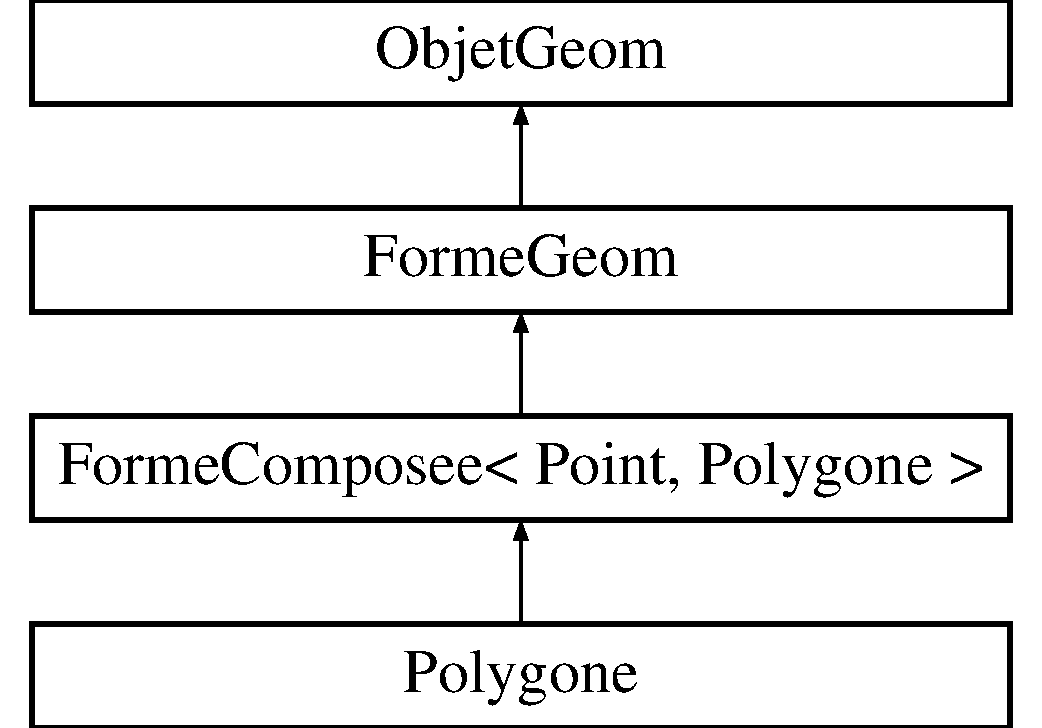
\includegraphics[height=4.000000cm]{class_polygone}
\end{center}
\end{figure}
\subsection*{Fonctions membres publiques}
\begin{DoxyCompactItemize}
\item 
\hypertarget{class_polygone_a2b5e7a67425d3c6e6f0b4d0c998928ae}{{\bfseries Polygone} (const Couleurs\+::\+Couleur \&couleur, const \hyperlink{class_point}{Point} \&p1, const \hyperlink{class_point}{Point} \&p2, const \hyperlink{class_point}{Point} \&p3)}\label{class_polygone_a2b5e7a67425d3c6e6f0b4d0c998928ae}

\item 
\hypertarget{class_polygone_ad5dd11ef57a4955446e3d47c90c9a801}{{\bfseries Polygone} (const \hyperlink{class_point}{Point} \&p1, const \hyperlink{class_point}{Point} \&p2, const \hyperlink{class_point}{Point} \&p3)}\label{class_polygone_ad5dd11ef57a4955446e3d47c90c9a801}

\item 
\hypertarget{class_polygone_a1aef610ad14c85f49e2557d4104cfbc0}{{\bfseries Polygone} (const \hyperlink{class_forme_composee}{Forme\+Composee}$<$ \hyperlink{class_point}{Point}, \hyperlink{class_polygone}{Polygone} $>$ \&f)}\label{class_polygone_a1aef610ad14c85f49e2557d4104cfbc0}

\item 
\hypertarget{class_polygone_a668cda1260040ee9d9a273e619e89c77}{{\bfseries Polygone} (const \hyperlink{class_polygone}{Polygone} \&p)}\label{class_polygone_a668cda1260040ee9d9a273e619e89c77}

\item 
void \hyperlink{class_polygone_a866ae8e0988baecdd582b22924986c9e}{ajouter\+Point} (const \hyperlink{class_point}{Point} \&p)
\begin{DoxyCompactList}\small\item\em ajouter\+Point \end{DoxyCompactList}\item 
\hypertarget{class_polygone_afc3b49ce264ac9351decd6a949ee4195}{void {\bfseries supprimer\+Dernier} ()}\label{class_polygone_afc3b49ce264ac9351decd6a949ee4195}

\item 
\hyperlink{class_point}{Point} $\ast$ \hyperlink{class_polygone_a7a10a1addd6e669b9657f72d6a3ac014}{get} (size\+\_\+t i) const 
\begin{DoxyCompactList}\small\item\em get \end{DoxyCompactList}\item 
\hypertarget{class_polygone_ab12c615571471004936009f198a8ce2e}{virtual string {\bfseries to\+String} () const }\label{class_polygone_ab12c615571471004936009f198a8ce2e}

\item 
\hypertarget{class_polygone_a933d95c281ba00ce39baf52fe3063b5e}{virtual double {\bfseries aire} () const }\label{class_polygone_a933d95c281ba00ce39baf52fe3063b5e}

\item 
\hypertarget{class_polygone_af9ae1d761d5a7f6834e46138eddd925f}{virtual \hyperlink{class_polygone}{Polygone} $\ast$ {\bfseries clone} () const }\label{class_polygone_af9ae1d761d5a7f6834e46138eddd925f}

\item 
\hypertarget{class_polygone_a1715df4b7ffd9b1e983c082d5d61c1ab}{virtual void {\bfseries dessin} (const \hyperlink{class_dessinable}{Dessinable} \&) const }\label{class_polygone_a1715df4b7ffd9b1e983c082d5d61c1ab}

\item 
\hypertarget{class_polygone_ae293043ea9d180259771515a6496cd8c}{virtual \hyperlink{class_polygone_ae293043ea9d180259771515a6496cd8c}{$\sim$\+Polygone} ()}\label{class_polygone_ae293043ea9d180259771515a6496cd8c}

\begin{DoxyCompactList}\small\item\em \hyperlink{class_polygone_ae293043ea9d180259771515a6496cd8c}{Polygone\+::$\sim$\+Polygone} On doit supprimer les membres du vector car il s'agit de copies créées par l'instance. \end{DoxyCompactList}\end{DoxyCompactItemize}
\subsection*{Membres hérités additionnels}


\subsection{Description détaillée}
The \hyperlink{class_polygone}{Polygone} class Cette classe représente un poygone, c'est à dire une ensemble de points dans un ordre donné. Un polygone contient au moins trois points. Les points stockés dans un polygone sont des copies des points envoyés. L'ordre dans lequel on ajoute les points correspond à l'ordre dans lequel ils seront reliés\+: si on insère un point dans un polygone, il sera relié à au dernier point inséré et au premier de la liste. 

\subsection{Documentation des fonctions membres}
\hypertarget{class_polygone_a866ae8e0988baecdd582b22924986c9e}{\index{Polygone@{Polygone}!ajouter\+Point@{ajouter\+Point}}
\index{ajouter\+Point@{ajouter\+Point}!Polygone@{Polygone}}
\subsubsection[{ajouter\+Point}]{\setlength{\rightskip}{0pt plus 5cm}void Polygone\+::ajouter\+Point (
\begin{DoxyParamCaption}
\item[{const {\bf Point} \&}]{p}
\end{DoxyParamCaption}
)\hspace{0.3cm}{\ttfamily [inline]}}}\label{class_polygone_a866ae8e0988baecdd582b22924986c9e}


ajouter\+Point 


\begin{DoxyParams}{Paramètres}
{\em p} & Ajoute un point à la suite des précédents. Le point est stocké sous forme du pointeur d'une copie du point passé en paramètres. \\
\hline
\end{DoxyParams}
\hypertarget{class_polygone_a7a10a1addd6e669b9657f72d6a3ac014}{\index{Polygone@{Polygone}!get@{get}}
\index{get@{get}!Polygone@{Polygone}}
\subsubsection[{get}]{\setlength{\rightskip}{0pt plus 5cm}{\bf Point} $\ast$ Polygone\+::get (
\begin{DoxyParamCaption}
\item[{size\+\_\+t}]{i}
\end{DoxyParamCaption}
) const\hspace{0.3cm}{\ttfamily [inline]}}}\label{class_polygone_a7a10a1addd6e669b9657f72d6a3ac014}


get 


\begin{DoxyParams}{Paramètres}
{\em i} & \\
\hline
\end{DoxyParams}
\begin{DoxyReturn}{Renvoie}
Une copie du point à la position demandée, ou N\+U\+L\+L si i est incorrect. 
\end{DoxyReturn}


La documentation de cette classe a été générée à partir des fichiers suivants \+:\begin{DoxyCompactItemize}
\item 
polygone.\+h\item 
polygone.\+cpp\end{DoxyCompactItemize}

\hypertarget{class_segment}{\section{Référence de la classe Segment}
\label{class_segment}\index{Segment@{Segment}}
}
Graphe d'héritage de Segment\+:\begin{figure}[H]
\begin{center}
\leavevmode
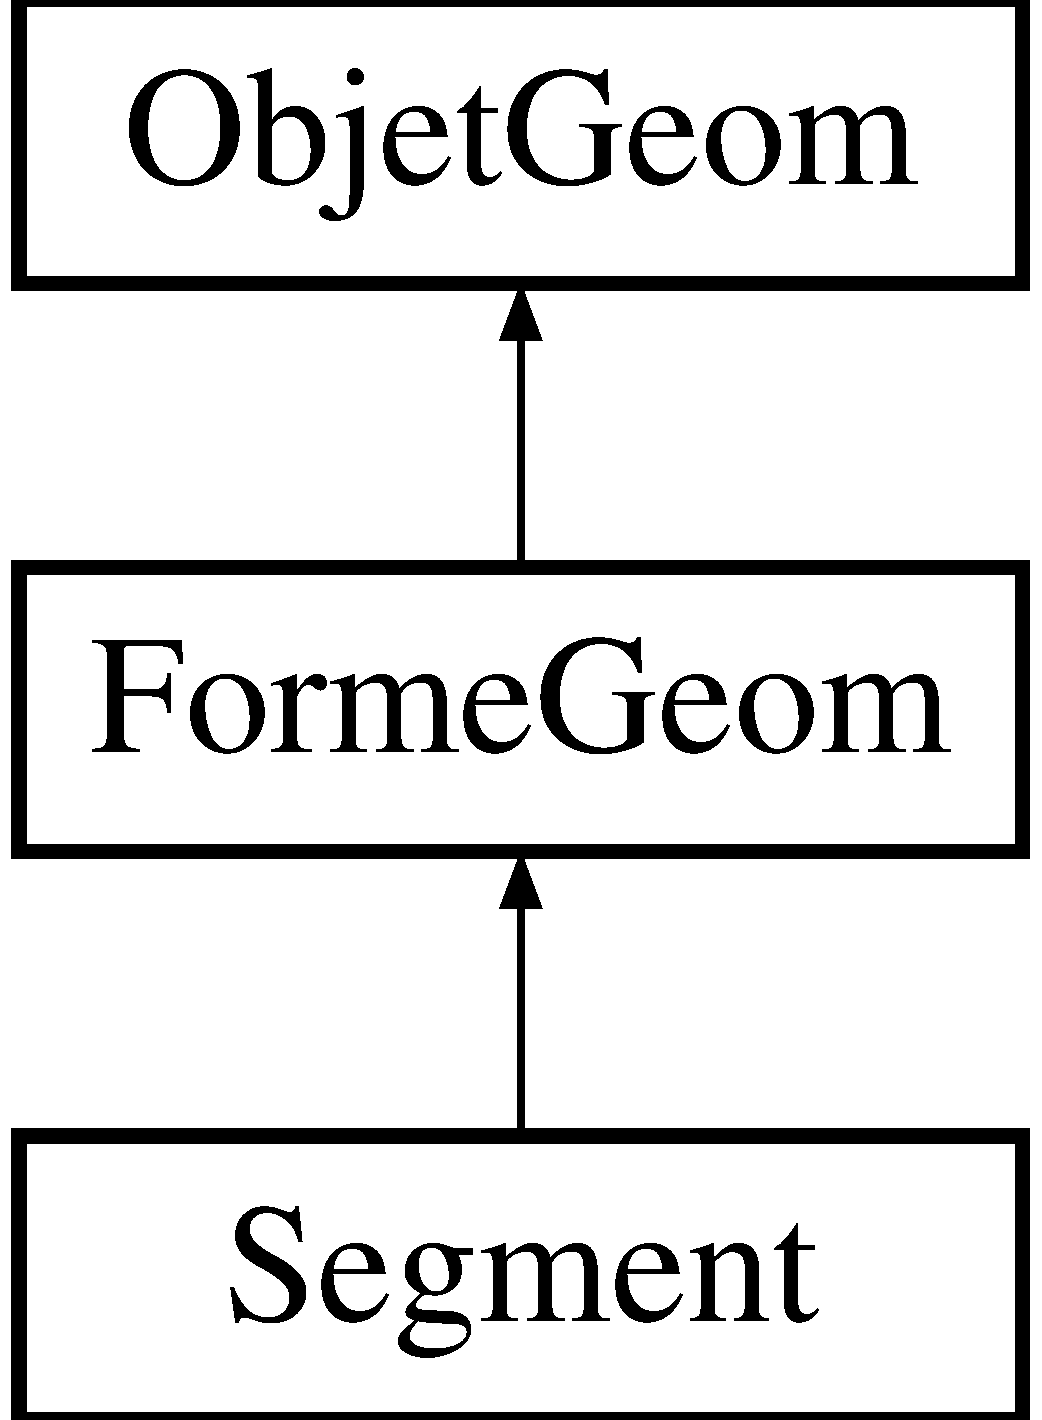
\includegraphics[height=3.000000cm]{class_segment}
\end{center}
\end{figure}
\subsection*{Fonctions membres publiques}
\begin{DoxyCompactItemize}
\item 
\hypertarget{class_segment_a865329de55a466d2ed10d092c0c5a45c}{{\bfseries Segment} (const Couleurs\+::\+Couleur \&couleur, const \hyperlink{class_point}{Point} \&p, const \hyperlink{class_point}{Point} \&p2)}\label{class_segment_a865329de55a466d2ed10d092c0c5a45c}

\item 
\hypertarget{class_segment_ab38dc6686cba332ad3a4200c391f0a1a}{{\bfseries Segment} (const \hyperlink{class_point}{Point} \&p, const \hyperlink{class_point}{Point} \&p2)}\label{class_segment_ab38dc6686cba332ad3a4200c391f0a1a}

\item 
\hypertarget{class_segment_ae51cb5320a024cdf469de58dc01529c4}{\hyperlink{class_point}{Point} {\bfseries get\+Point1} () const }\label{class_segment_ae51cb5320a024cdf469de58dc01529c4}

\item 
\hypertarget{class_segment_a7e7329612c9a022775b6e82678b7b1c1}{\hyperlink{class_point}{Point} {\bfseries get\+Point2} () const }\label{class_segment_a7e7329612c9a022775b6e82678b7b1c1}

\item 
\hypertarget{class_segment_a0a3105557d1d22b5fbecd4b5aef5a49f}{virtual string {\bfseries to\+String} () const }\label{class_segment_a0a3105557d1d22b5fbecd4b5aef5a49f}

\item 
\hypertarget{class_segment_ab180d3d792d6a4a58decc85e596cfd2b}{virtual \hyperlink{class_segment}{Segment} $\ast$ {\bfseries rotation} (const \hyperlink{class_point}{Point} \&p, const \hyperlink{class_angle}{Angle} \&angle) const }\label{class_segment_ab180d3d792d6a4a58decc85e596cfd2b}

\item 
\hypertarget{class_segment_ae83d6693cd1444b75cbb001ae730a703}{virtual \hyperlink{class_segment}{Segment} $\ast$ {\bfseries homothetie} (const \hyperlink{class_point}{Point} \&p, const double \&scale) const }\label{class_segment_ae83d6693cd1444b75cbb001ae730a703}

\item 
\hypertarget{class_segment_af140a6dc21ac42ded1d427f43e875106}{virtual \hyperlink{class_segment}{Segment} $\ast$ {\bfseries translation} (const \hyperlink{class_vecteur}{Vecteur} \&v) const }\label{class_segment_af140a6dc21ac42ded1d427f43e875106}

\item 
\hypertarget{class_segment_a059d934ffa8d7427f16beb79ce8d794f}{virtual double {\bfseries aire} () const }\label{class_segment_a059d934ffa8d7427f16beb79ce8d794f}

\item 
\hypertarget{class_segment_ab664920d9164e81e5817b29ffc41d411}{virtual \hyperlink{class_segment}{Segment} $\ast$ {\bfseries clone} () const }\label{class_segment_ab664920d9164e81e5817b29ffc41d411}

\item 
\hypertarget{class_segment_a35991f2c6c2cb0db2a64802e3fd09984}{virtual void {\bfseries dessin} (const \hyperlink{class_dessinable}{Dessinable} \&) const }\label{class_segment_a35991f2c6c2cb0db2a64802e3fd09984}

\end{DoxyCompactItemize}
\subsection*{Membres hérités additionnels}


La documentation de cette classe a été générée à partir des fichiers suivants \+:\begin{DoxyCompactItemize}
\item 
segment.\+h\item 
segment.\+cpp\end{DoxyCompactItemize}

\hypertarget{class_triangle}{\section{Référence de la classe Triangle}
\label{class_triangle}\index{Triangle@{Triangle}}
}
Graphe d'héritage de Triangle\+:\begin{figure}[H]
\begin{center}
\leavevmode
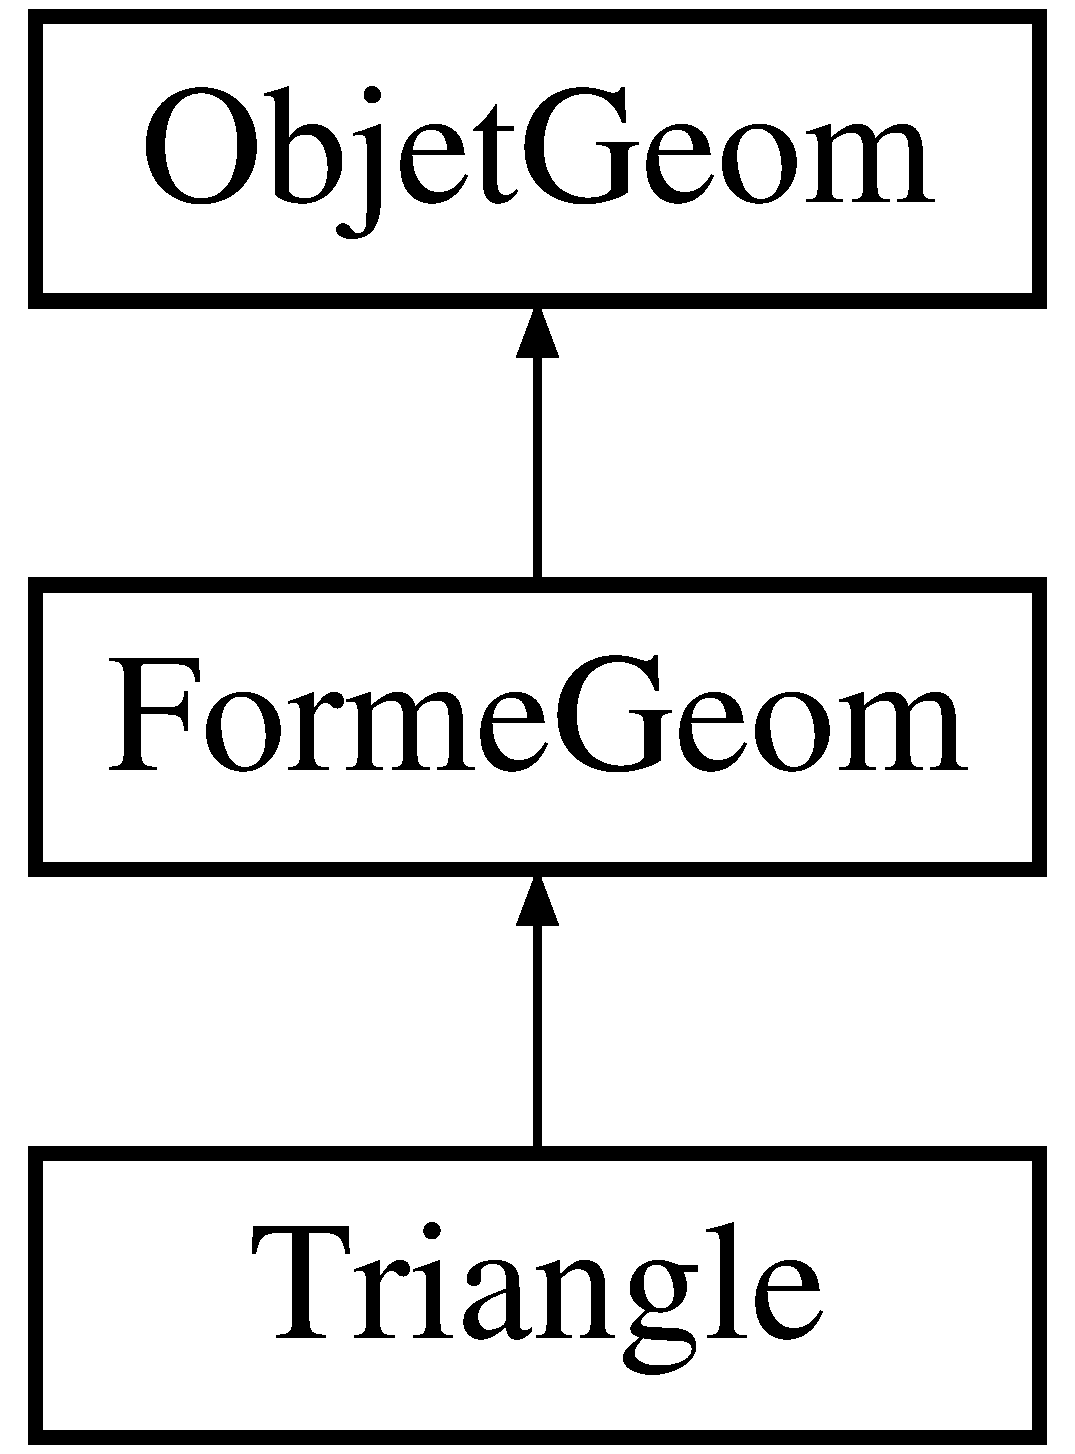
\includegraphics[height=3.000000cm]{class_triangle}
\end{center}
\end{figure}
\subsection*{Fonctions membres publiques}
\begin{DoxyCompactItemize}
\item 
\hypertarget{class_triangle_a96c1681b2b1752c7b4a75bce9c4855ab}{{\bfseries Triangle} (const \hyperlink{class_triangle}{Triangle} \&t)}\label{class_triangle_a96c1681b2b1752c7b4a75bce9c4855ab}

\item 
\hypertarget{class_triangle_a0fdb0e438429946040a288675c43a67f}{{\bfseries Triangle} (const \hyperlink{class_point}{Point} \&p1, const \hyperlink{class_point}{Point} \&p2, const \hyperlink{class_point}{Point} \&p3)}\label{class_triangle_a0fdb0e438429946040a288675c43a67f}

\item 
\hypertarget{class_triangle_a11fbd4b84d3e13385d330b17aec44a77}{{\bfseries Triangle} (const Couleurs\+::\+Couleur \&couleur, const \hyperlink{class_point}{Point} \&p1, const \hyperlink{class_point}{Point} \&p2, const \hyperlink{class_point}{Point} \&p3)}\label{class_triangle_a11fbd4b84d3e13385d330b17aec44a77}

\item 
\hypertarget{class_triangle_abdb0b754dfc0442c5514723d26a4c447}{\hyperlink{class_point}{Point} {\bfseries get\+P1} () const }\label{class_triangle_abdb0b754dfc0442c5514723d26a4c447}

\item 
\hypertarget{class_triangle_a5321f63dbe9adcda3bdf5065695ec7a5}{\hyperlink{class_point}{Point} {\bfseries get\+P2} () const }\label{class_triangle_a5321f63dbe9adcda3bdf5065695ec7a5}

\item 
\hypertarget{class_triangle_aa14eba0138f5250bca2dcc929eea064d}{\hyperlink{class_point}{Point} {\bfseries get\+P3} () const }\label{class_triangle_aa14eba0138f5250bca2dcc929eea064d}

\item 
\hypertarget{class_triangle_a2d989db970abfac992988e46bf615a3a}{virtual string {\bfseries to\+String} () const }\label{class_triangle_a2d989db970abfac992988e46bf615a3a}

\item 
\hypertarget{class_triangle_a32073e547daa9557f2361a9efc06d16a}{virtual \hyperlink{class_triangle}{Triangle} $\ast$ {\bfseries rotation} (const \hyperlink{class_point}{Point} \&p, const \hyperlink{class_angle}{Angle} \&angle) const }\label{class_triangle_a32073e547daa9557f2361a9efc06d16a}

\item 
\hypertarget{class_triangle_af5dd89e0b0533d31b95faae75d63651e}{virtual \hyperlink{class_triangle}{Triangle} $\ast$ {\bfseries homothetie} (const \hyperlink{class_point}{Point} \&p, const double \&scale) const }\label{class_triangle_af5dd89e0b0533d31b95faae75d63651e}

\item 
\hypertarget{class_triangle_a16a110eb05439c0deb557eacbc95ef65}{virtual \hyperlink{class_triangle}{Triangle} $\ast$ {\bfseries translation} (const \hyperlink{class_vecteur}{Vecteur} \&v) const }\label{class_triangle_a16a110eb05439c0deb557eacbc95ef65}

\item 
virtual double \hyperlink{class_triangle_ab8f3ee5da959716a0d08f5a1206ff8bf}{aire} () const 
\begin{DoxyCompactList}\small\item\em \hyperlink{class_triangle_ab8f3ee5da959716a0d08f5a1206ff8bf}{Triangle\+::aire} Calcule l'aire du triangle grâce à la méthode de Héron. \end{DoxyCompactList}\item 
\hypertarget{class_triangle_a1a1075e1000326f1776b10f2da4f428a}{virtual \hyperlink{class_triangle}{Triangle} $\ast$ {\bfseries clone} () const }\label{class_triangle_a1a1075e1000326f1776b10f2da4f428a}

\item 
\hypertarget{class_triangle_a4f18d46678287521615b1de2e805e69d}{virtual void {\bfseries dessin} (const \hyperlink{class_dessinable}{Dessinable} \&) const }\label{class_triangle_a4f18d46678287521615b1de2e805e69d}

\end{DoxyCompactItemize}
\subsection*{Membres hérités additionnels}


\subsection{Documentation des fonctions membres}
\hypertarget{class_triangle_ab8f3ee5da959716a0d08f5a1206ff8bf}{\index{Triangle@{Triangle}!aire@{aire}}
\index{aire@{aire}!Triangle@{Triangle}}
\subsubsection[{aire}]{\setlength{\rightskip}{0pt plus 5cm}double Triangle\+::aire (
\begin{DoxyParamCaption}
{}
\end{DoxyParamCaption}
) const\hspace{0.3cm}{\ttfamily [virtual]}}}\label{class_triangle_ab8f3ee5da959716a0d08f5a1206ff8bf}


\hyperlink{class_triangle_ab8f3ee5da959716a0d08f5a1206ff8bf}{Triangle\+::aire} Calcule l'aire du triangle grâce à la méthode de Héron. 

\begin{DoxyReturn}{Renvoie}
l'aire 
\end{DoxyReturn}


Implémente \hyperlink{class_forme_geom}{Forme\+Geom}.



La documentation de cette classe a été générée à partir des fichiers suivants \+:\begin{DoxyCompactItemize}
\item 
triangle.\+h\item 
triangle.\+cpp\end{DoxyCompactItemize}

\hypertarget{class_vecteur}{\section{Référence de la classe Vecteur}
\label{class_vecteur}\index{Vecteur@{Vecteur}}
}
\subsection*{Fonctions membres publiques}
\begin{DoxyCompactItemize}
\item 
\hypertarget{class_vecteur_a46d3489a12a0233448648651532607ff}{{\bfseries Vecteur} (const double \&x=0, const double \&y=0)}\label{class_vecteur_a46d3489a12a0233448648651532607ff}

\item 
\hypertarget{class_vecteur_a95e860a6f134384a5ae870c1960e54b6}{{\bfseries Vecteur} (const \hyperlink{class_point}{Point} \&p1, const \hyperlink{class_point}{Point} \&p2)}\label{class_vecteur_a95e860a6f134384a5ae870c1960e54b6}

\item 
\hypertarget{class_vecteur_a5b328da1ba17bca82048359d59c0abc3}{{\bfseries Vecteur} (const \hyperlink{class_vecteur}{Vecteur} \&v1, const \hyperlink{class_vecteur}{Vecteur} \&v2)}\label{class_vecteur_a5b328da1ba17bca82048359d59c0abc3}

\item 
\hypertarget{class_vecteur_a42f7a7f1dc44e088c278d3b3363c5a33}{double {\bfseries get\+X} () const }\label{class_vecteur_a42f7a7f1dc44e088c278d3b3363c5a33}

\item 
\hypertarget{class_vecteur_a323d689fb951261b557ea65b10af3893}{double {\bfseries get\+Y} () const }\label{class_vecteur_a323d689fb951261b557ea65b10af3893}

\item 
\hyperlink{class_vecteur}{Vecteur} \hyperlink{class_vecteur_a9d61176ddcefcc1dcf0ae2d5fd2e9ee7}{rotation} (const \hyperlink{class_vecteur}{Vecteur} \&p, const \hyperlink{class_angle}{Angle} \&a) const 
\begin{DoxyCompactList}\small\item\em \hyperlink{class_point_a32bc5c9d0e07f0e4b54187ffcd3c8a67}{Point\+::rotation}. \end{DoxyCompactList}\item 
\hypertarget{class_vecteur_ab012afb15826a7d5858a3b45ea763a57}{\hyperlink{class_vecteur}{Vecteur} {\bfseries homothetie} (const \hyperlink{class_vecteur}{Vecteur} \&p, double scale) const }\label{class_vecteur_ab012afb15826a7d5858a3b45ea763a57}

\item 
\hypertarget{class_vecteur_ae748a1c896716a7983e53e1dbfdbb815}{bool {\bfseries operator==} (const \hyperlink{class_vecteur}{Vecteur} \&v) const }\label{class_vecteur_ae748a1c896716a7983e53e1dbfdbb815}

\item 
\hypertarget{class_vecteur_ae22b87d8ad6628b235bed15de8d8aaa2}{const \hyperlink{class_vecteur}{Vecteur} {\bfseries operator+} (const \hyperlink{class_vecteur}{Vecteur} \&v) const }\label{class_vecteur_ae22b87d8ad6628b235bed15de8d8aaa2}

\item 
\hypertarget{class_vecteur_ac01814448a6ecce07a03088c00504fb0}{const \hyperlink{class_vecteur}{Vecteur} {\bfseries operator-\/} (const \hyperlink{class_vecteur}{Vecteur} \&v) const }\label{class_vecteur_ac01814448a6ecce07a03088c00504fb0}

\item 
\hypertarget{class_vecteur_a45870b151569e48d0286ad2761e4c655}{double {\bfseries operator$\ast$} (const \hyperlink{class_vecteur}{Vecteur} \&v) const }\label{class_vecteur_a45870b151569e48d0286ad2761e4c655}

\item 
\hypertarget{class_vecteur_a5b537a840a32a9399456bc8a65b2f7ed}{const \hyperlink{class_vecteur}{Vecteur} {\bfseries operator$\ast$} (const double \&a) const }\label{class_vecteur_a5b537a840a32a9399456bc8a65b2f7ed}

\item 
\hypertarget{class_vecteur_a1b5f3856ab3c36ab39a168a9ba92accb}{const \hyperlink{class_vecteur}{Vecteur} {\bfseries operator-\/} () const }\label{class_vecteur_a1b5f3856ab3c36ab39a168a9ba92accb}

\item 
\hypertarget{class_vecteur_afa6e8ccd9771f87419077954cf96677a}{double {\bfseries norme} () const }\label{class_vecteur_afa6e8ccd9771f87419077954cf96677a}

\item 
\hypertarget{class_vecteur_a98103b18e3e8529e6d5f600689d67833}{{\bfseries operator std\+::string} () const }\label{class_vecteur_a98103b18e3e8529e6d5f600689d67833}

\end{DoxyCompactItemize}


\subsection{Documentation des fonctions membres}
\hypertarget{class_vecteur_a9d61176ddcefcc1dcf0ae2d5fd2e9ee7}{\index{Vecteur@{Vecteur}!rotation@{rotation}}
\index{rotation@{rotation}!Vecteur@{Vecteur}}
\subsubsection[{rotation}]{\setlength{\rightskip}{0pt plus 5cm}{\bf Vecteur} Vecteur\+::rotation (
\begin{DoxyParamCaption}
\item[{const {\bf Vecteur} \&}]{p, }
\item[{const {\bf Angle} \&}]{a}
\end{DoxyParamCaption}
) const}}\label{class_vecteur_a9d61176ddcefcc1dcf0ae2d5fd2e9ee7}


\hyperlink{class_point_a32bc5c9d0e07f0e4b54187ffcd3c8a67}{Point\+::rotation}. 


\begin{DoxyParams}{Paramètres}
{\em p} & le point à partir duquel il faut effectuer la rotation \\
\hline
{\em a} & l'angle de la rotation \\
\hline
\end{DoxyParams}
\begin{DoxyReturn}{Renvoie}
le point résultat Permet de calculer le point issus de la rotation du point courrant par rapport à p et a 
\end{DoxyReturn}


La documentation de cette classe a été générée à partir des fichiers suivants \+:\begin{DoxyCompactItemize}
\item 
vecteur.\+h\item 
vecteur.\+cpp\end{DoxyCompactItemize}

%--- End generated contents ---

% Index
\newpage
\phantomsection
\addcontentsline{toc}{chapter}{Index}
\printindex

\end{document}
